\documentclass{beamer}
\usetheme{}
\usecolortheme{dolphin}           
\useinnertheme{circles}
\setbeamertemplate{itemize items}[default]
\setbeamertemplate{enumerate items}[default]
\usepackage[T1]{fontenc}
\usepackage[utf8]{inputenc}
\usepackage{lmodern}
\usepackage{amsmath}
\usepackage{booktabs} 
\usepackage{graphicx}        
\usepackage{array}
\usepackage{color}
\makeatletter
\def\zapcolorreset{\let\reset@color\relax\ignorespaces}
\def\colorrows#1{\noalign{\aftergroup\zapcolorreset#1}\ignorespaces}
\makeatother
\setbeamertemplate{navigation symbols}{}
\setbeamertemplate{footline}[frame number]

%--------------------------------------
\title{Economic growth}
\author{School of Economics, University College Dublin}
\date{Spring 2018}
\begin{document}

%--------------------------------------
\begin{frame}
 \titlepage
\end{frame}
%--------------------------------------

%--------------------------------------
\begin{frame}
  Broadly speaking the EU has two main aims
  \begin{enumerate}
    \item Ensure political stability
    \item Improve living standards
  \end{enumerate}
\end{frame}
%--------------------------------------

%--------------------------------------
\begin{frame}
  Within EU framework number of factors that affect economic growth
  \begin{enumerate}
    \item International factors
    \begin{itemize}
      \item Exchange rate regimes; terms of trade; capital flows
    \end{itemize}
    \item Policy
    \begin{itemize}
      \item Promoting competitiveness; full employment; work quality; social cohesion; innovation
    \end{itemize}
  \end{enumerate}
\end{frame}
%--------------------------------------

%--------------------------------------
\begin{frame}
 \textbf{Cobb-Douglas function}\\
 Useful to examine factors that contribute to growth
\begin{align}
  Y_t=A_tK^{\alpha}_tL^{\beta}_t
\end{align}
$K$ is capital\\
$L$ labour\\
$A$ accounts for technology. 
\end{frame}
%--------------------------------------

%--------------------------------------
\begin{frame}
 Technology is an important source of growth
\begin{itemize}
  \item Increase in $A_t$ results in higher output without having to raise inputs
  \item Measure of productive efficiency
  \item Can fluctuate for various reasons, e.g. new technology, government regulation, management style
\end{itemize}
  Since an increase in $A_t$ increases productiveness of other factors it is also known as \textbf{Total Factor Productivity} (TFP).
\end{frame}
%--------------------------------------

%--------------------------------------
\begin{frame}
 \textbf{Productivity}\\
 Often interested in output per worker; can re-write (1)
 \begin{align}
  \frac{Y_t}{L_t}= A_t \left(\frac{K_t}{L_t} \right)^{\alpha}L_t^{\alpha + \beta -1}
 \end{align}
 \medskip
 Shows three potential ways to increase productivity
 \begin{enumerate}
   \item Increase in number of workers
   \item Capital deepening
   \item Technological progress
 \end{enumerate}
\end{frame}
%--------------------------------------

%--------------------------------------
\begin{frame}
  \textbf{More workers} will only add to growth when
  \begin{align}
    \alpha+\beta>1
  \end{align}
  \medskip
  Most growth theories assume constant returns to scale
  \begin{align}
    \beta=1-\alpha
  \end{align}
  Production function becomes
  \begin{align}
    \frac{Y_t}{L_t}= A_t \left(\frac{K_t}{L_t} \right)^{\alpha}
  \end{align}
\end{frame}
%--------------------------------------

%--------------------------------------
\begin{frame}
  \textbf{Swan-Solow model} links output to capital, labour and technological efficieny parameter
  \begin{align}
    Y_t = AF(K_t,L_t) 
  \end{align}
  Key feature is diminishing marginal return to capital accumulation
  \begin{itemize}
    \item Increase in $K$ will give progressively smaller increase in $Y$
    \begin{align}
       \frac{\delta^2Y_t}{\delta K_t}<0    
    \end{align}
    \item Assuming constant labour supply
  \end{itemize}
\end{frame}
%--------------------------------------

%--------------------------------------
\begin{frame}
  Model assumes closed economy and no government sector
  \begin{itemize}
    \item No international trade or public spending
  \end{itemize}
  \medskip
  All output takes form of consumption or investment
  \begin{align}
       Y_t &= C_t+I_t\\
       S_t &= Y_t-C_t=I_t
  \end{align}
  \medskip
  Capital depreciates
\begin{align*}
  \frac{\partial K_t}{\partial t}=I_t -\gamma K_t
\end{align*}
Capital stock depends on 
\begin{itemize}
  \item Investments (+)
  \item Depreciation rate (-)
\end{itemize}
\end{frame}
%--------------------------------------

%--------------------------------------
\begin{frame}
  Consumers save constant share of income: investments will be constant fraction of output
\begin{align}
  S_t = sY_t = I_t
\end{align}
Investment level is given by
\begin{align}
  I_t=sY_t=sAF(K_t,L_t)
\end{align}
 \textbf{NB-} One off increase in technology level $A$ has the same effect as a one off increase in $s$ 
 \begin{itemize}
   \item Capital and output gradually increase to a new level
 \end{itemize}
\end{frame}
%--------------------------------------

%--------------------------------------
\begin{frame}
  \textbf{$K$ vs. $A$}\\
  Important difference between two determinants of growth
  \begin{itemize}
    \item Savings rate $s$ is subject to a limit
    \item $A$ does not face constraints. 
  \end{itemize}
  \medskip
  Implication: for long-term sustainable growth TFP increases matter
  \begin{itemize}
    \item Growth through capital accumulation will taper off over time producing a one-off increase in output per worker whereas TFP growth can lead to sustained higher growth rates of output per worker
  \end{itemize}
\end{frame}
%--------------------------------------

%--------------------------------------
\begin{frame}
  How well are EU countries doing in terms of economic growth?
  \begin{itemize}
    \item Recall situation was pretty bleak following WW2
  \end{itemize}
  \medskip
  Answering this question can take two approaches  
\begin{enumerate}
  \item US comparison
  \item Development of new EU member states
\end{enumerate}
\end{frame}
%--------------------------------------

%--------------------------------------
\begin{frame}
  \begin{figure}
    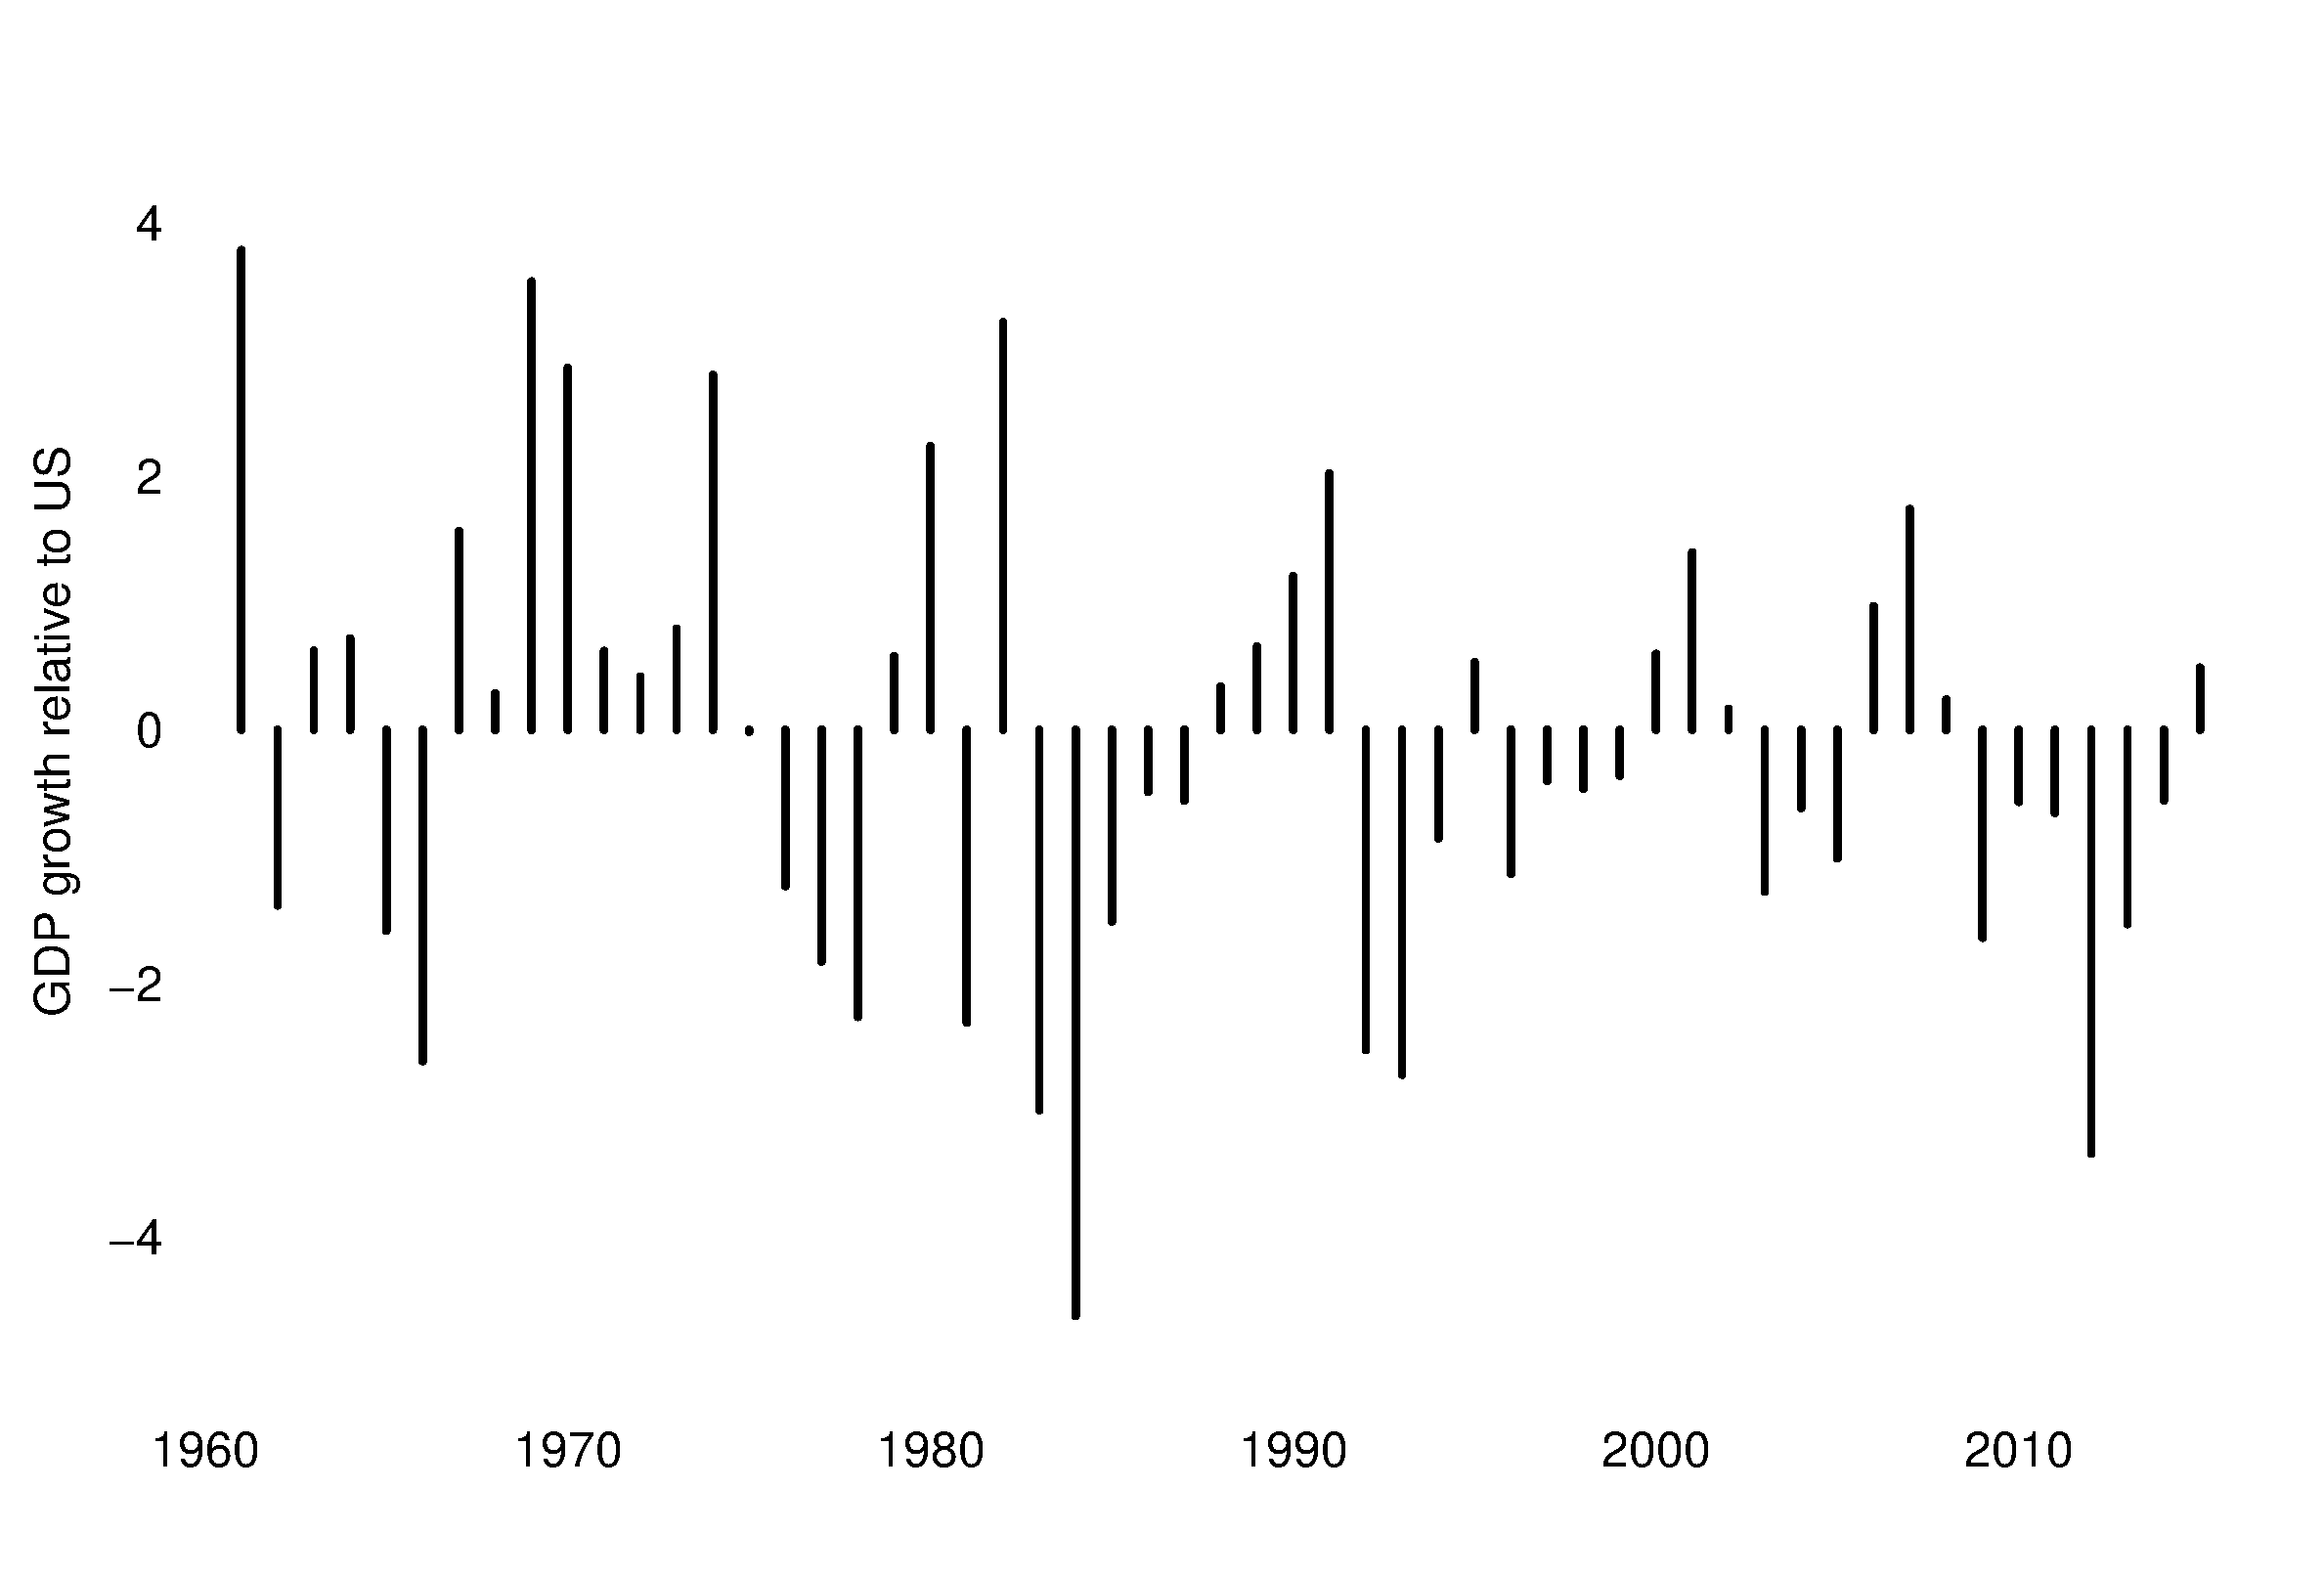
\includegraphics[scale=.3]{versus_us.eps}
  \end{figure}
\end{frame}
%--------------------------------------

%--------------------------------------
\begin{frame}
  \begin{figure}
    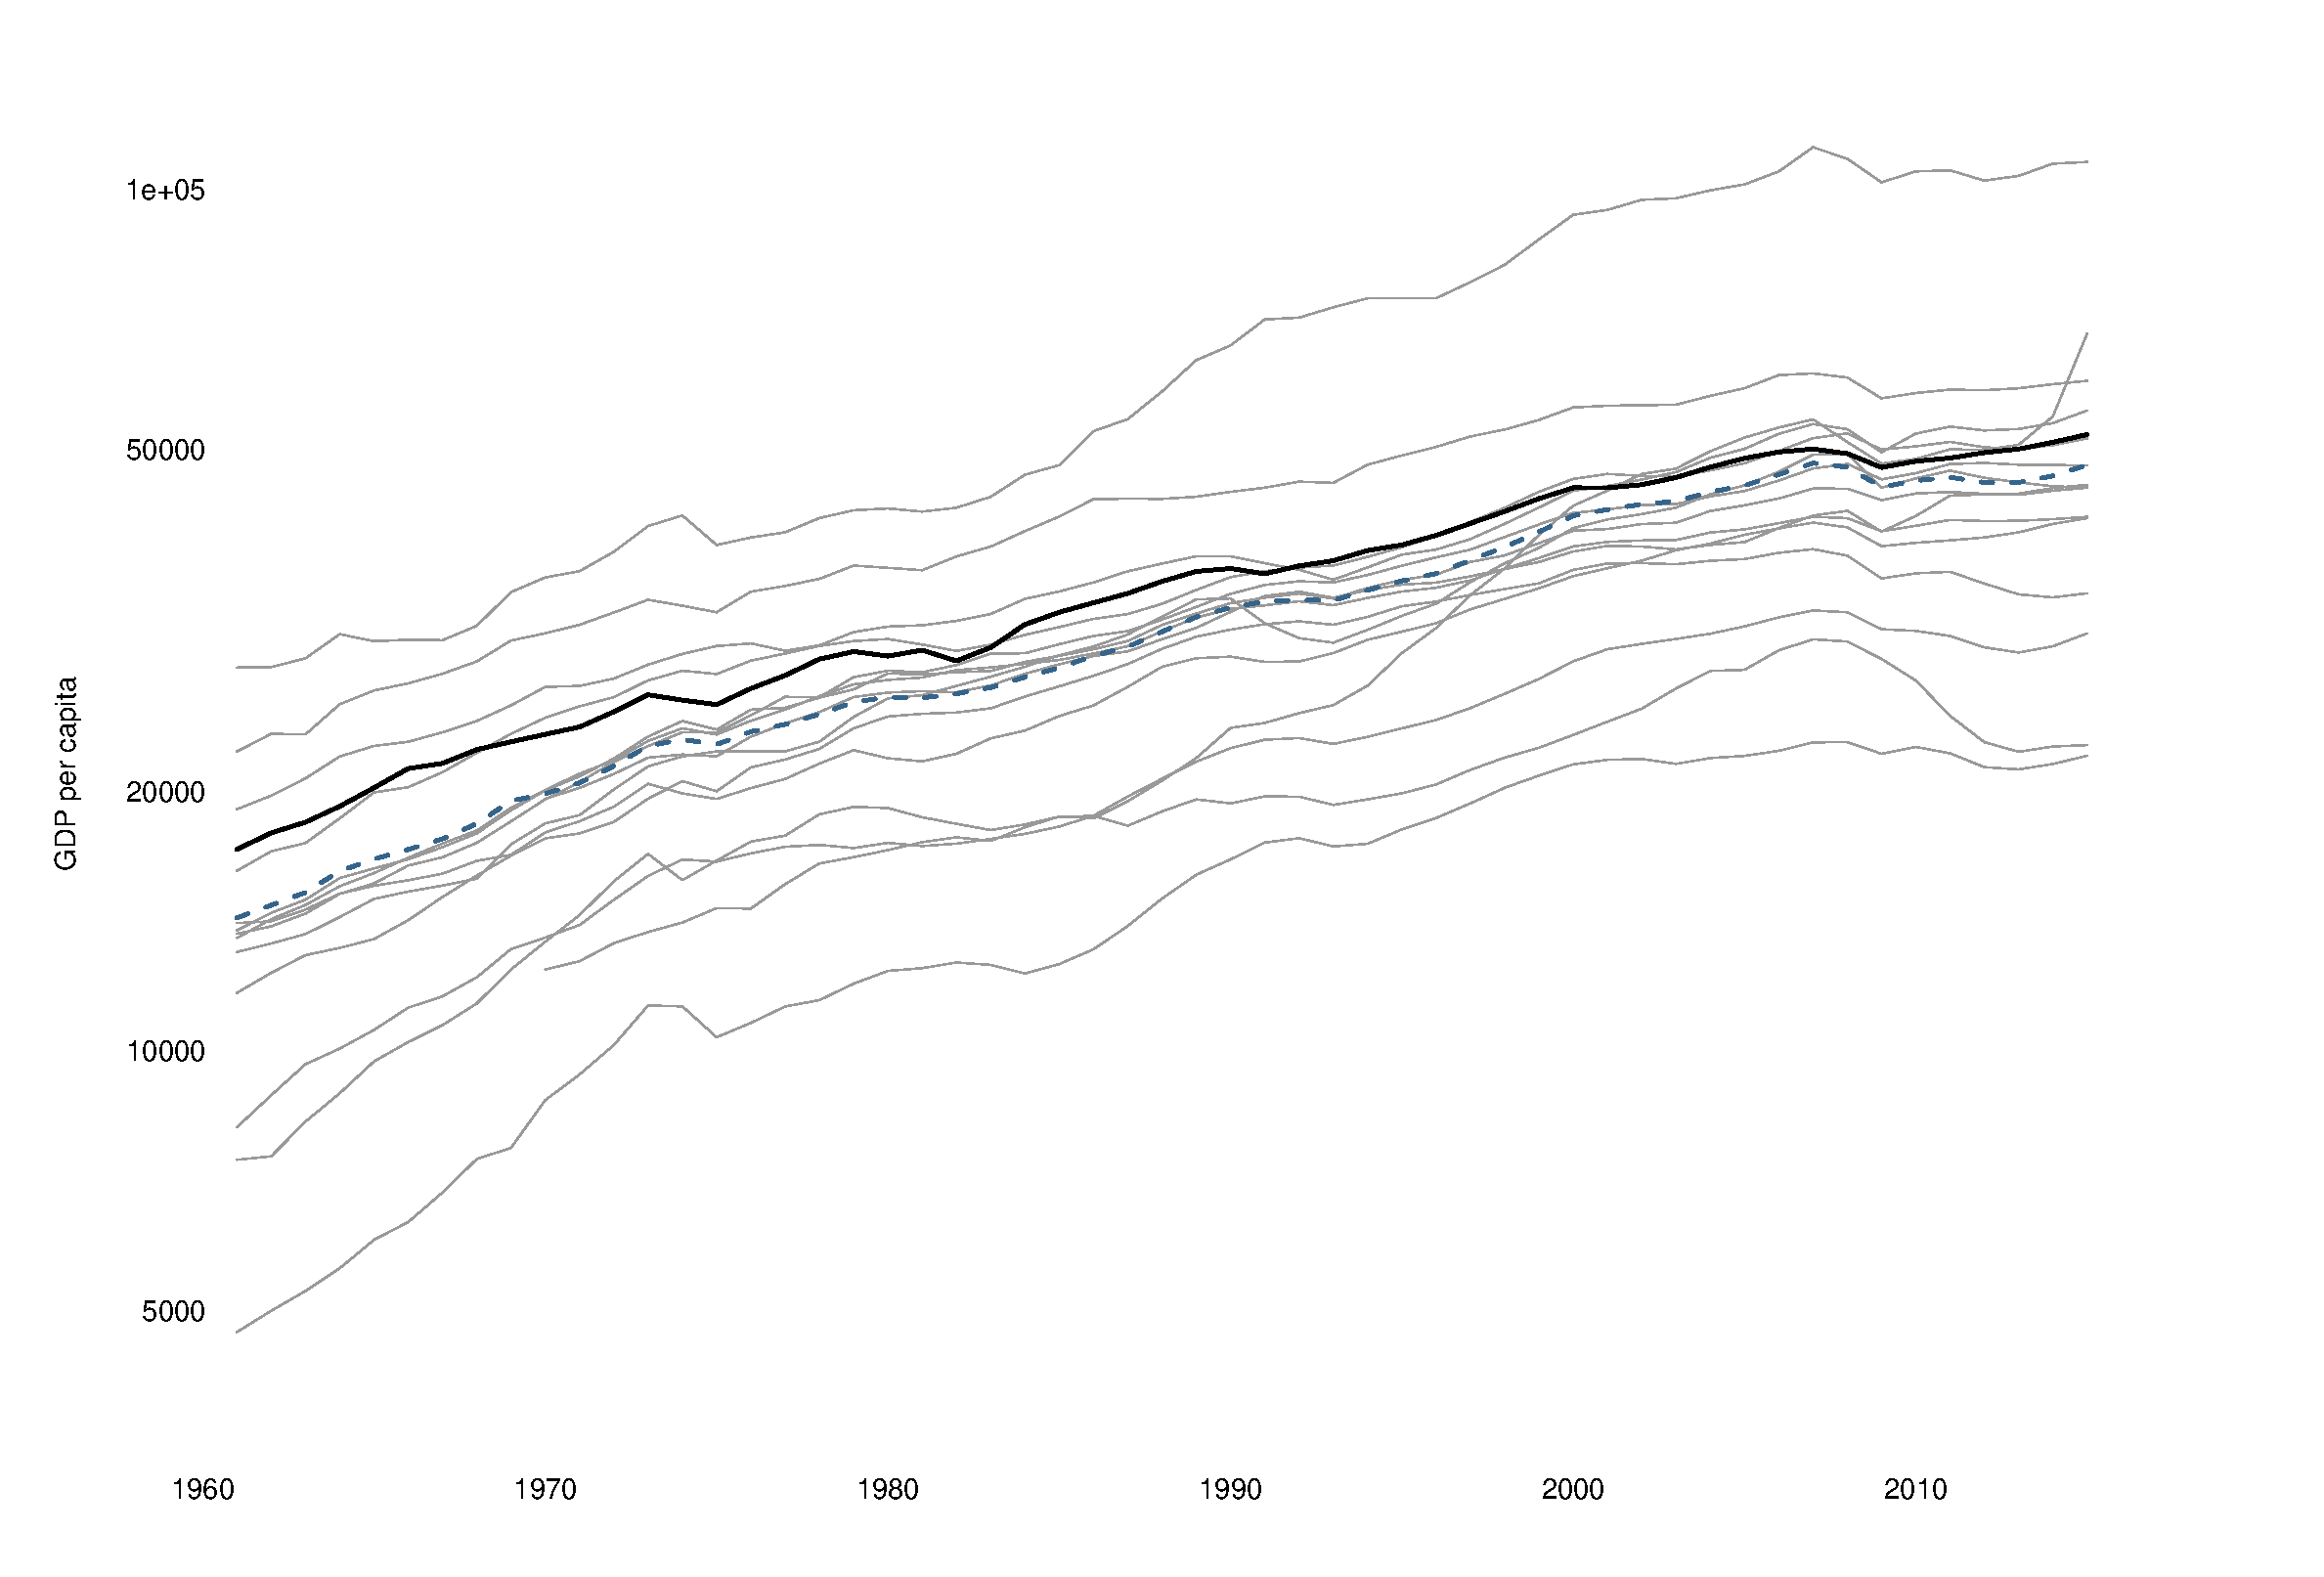
\includegraphics[scale=.3]{versus_us2.eps}
  \end{figure}
\end{frame}
%--------------------------------------

%--------------------------------------
\begin{frame}
  \begin{figure}
    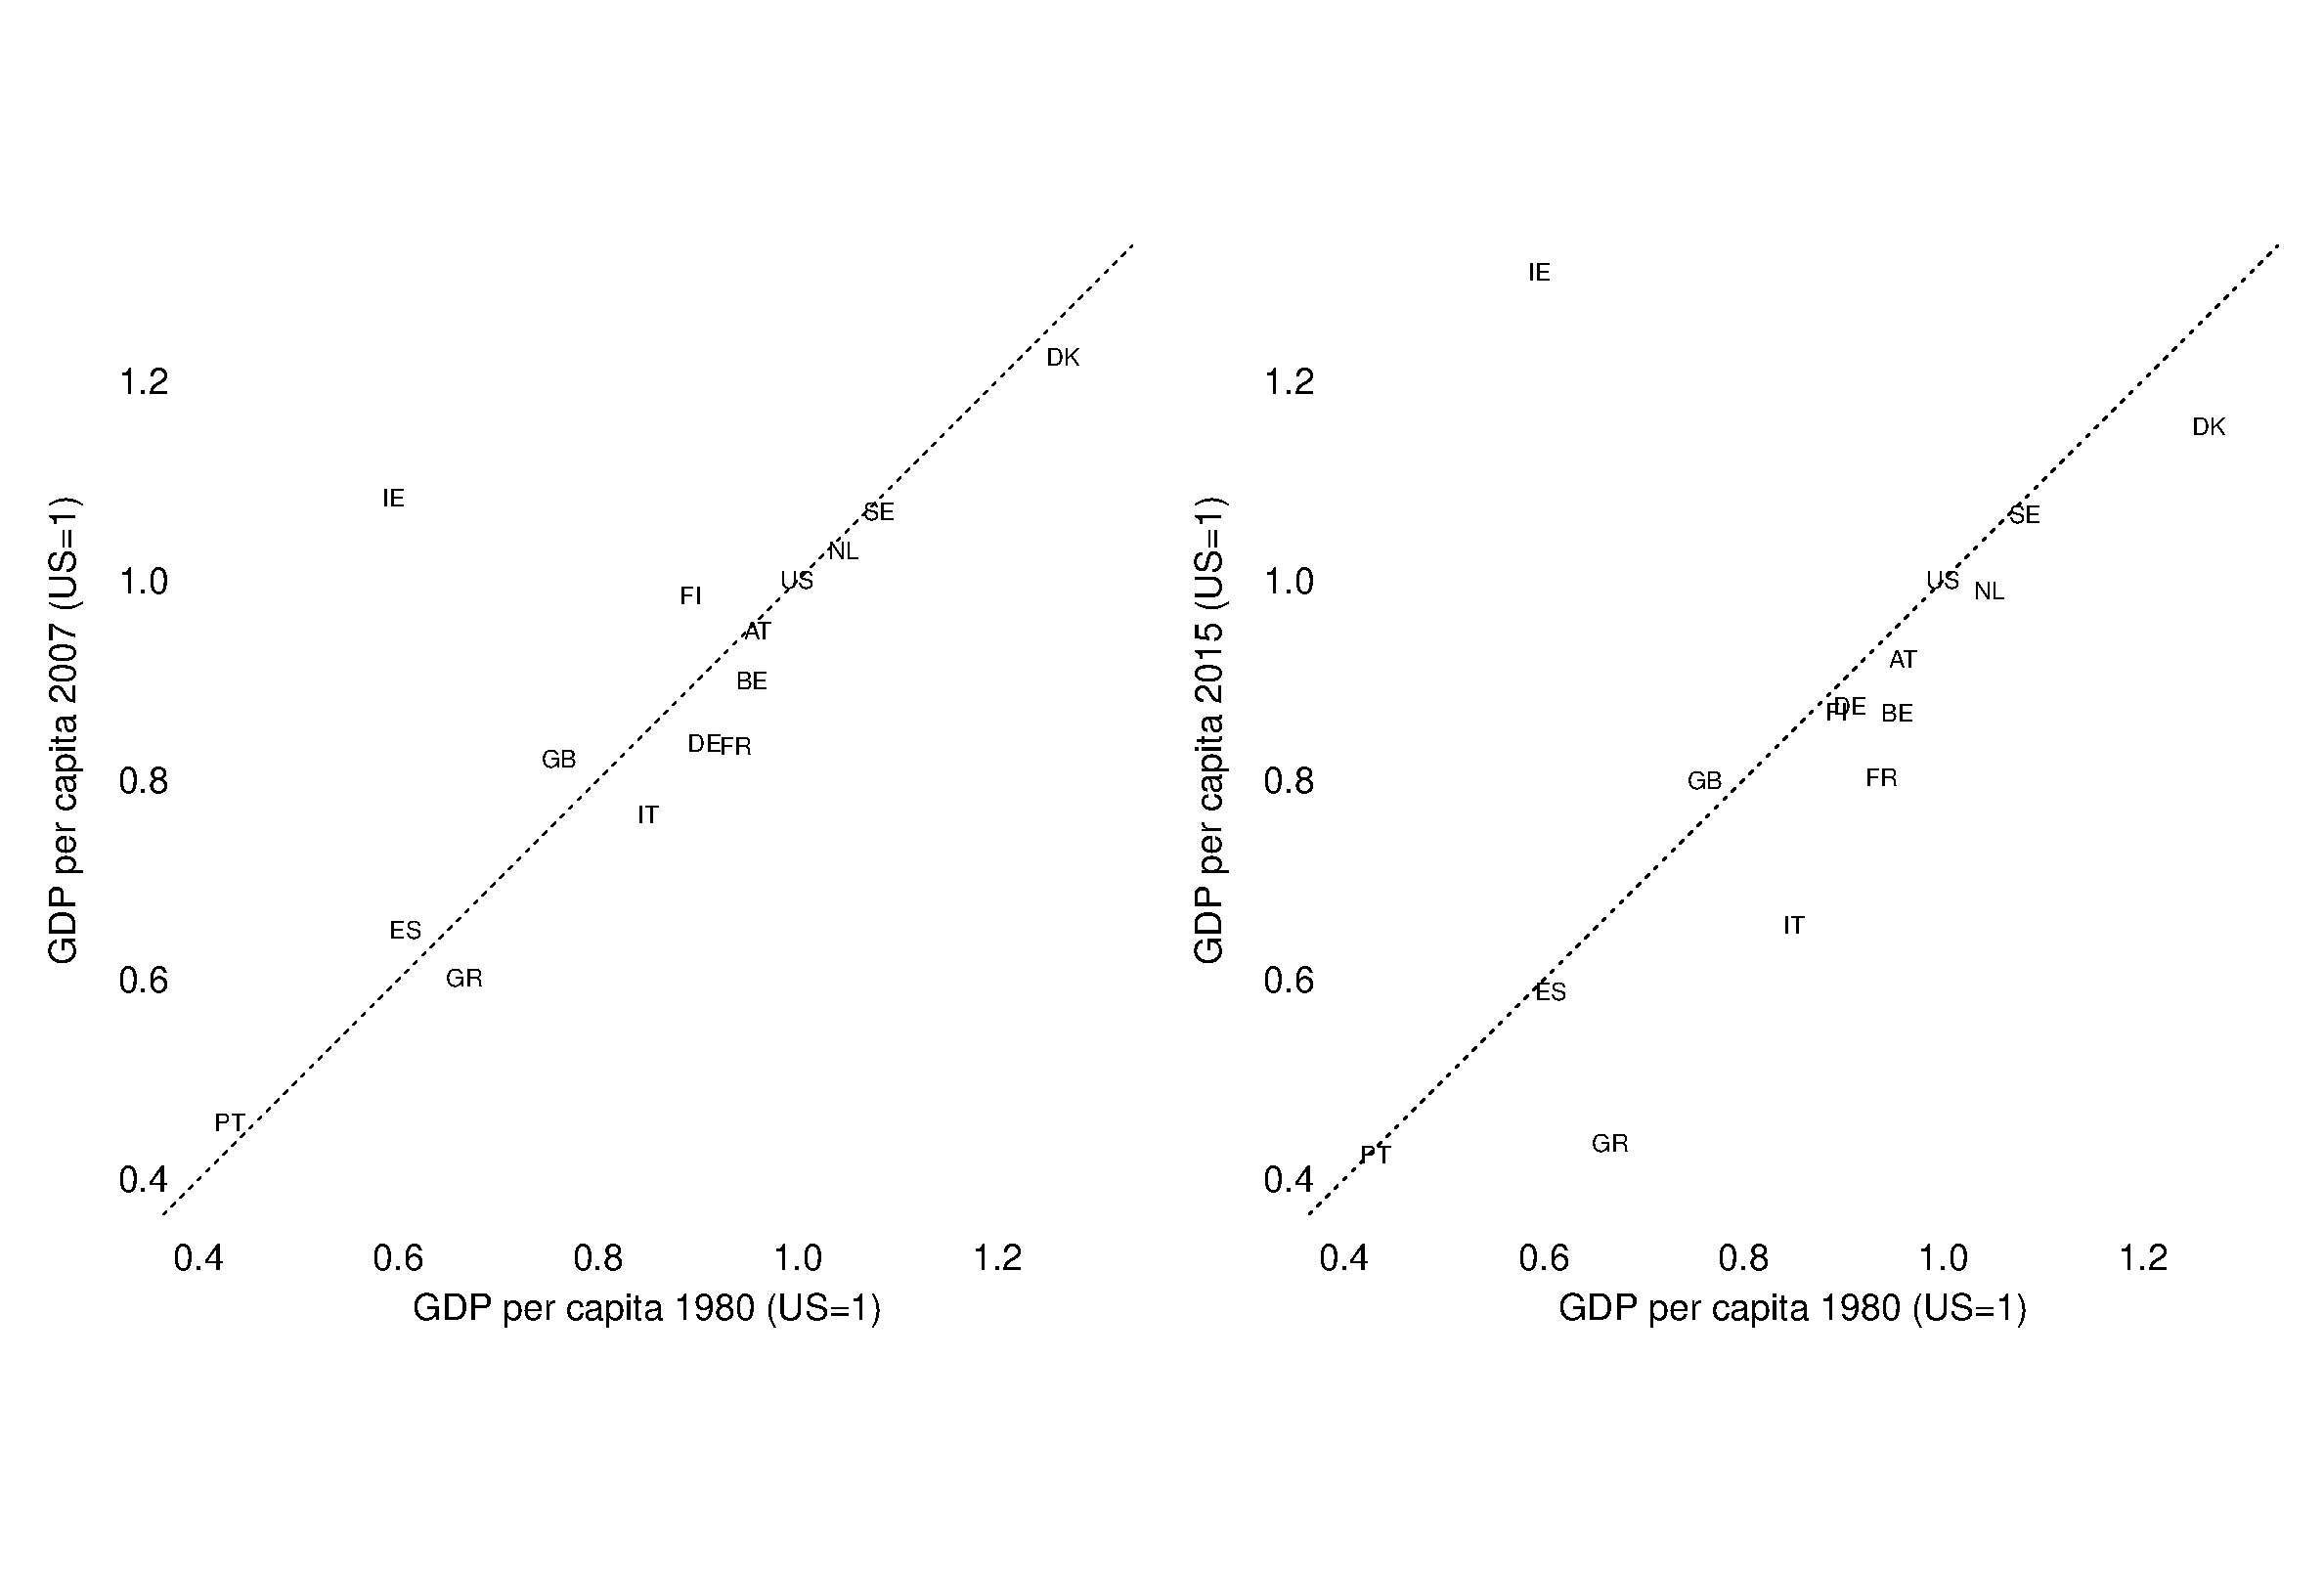
\includegraphics[scale=.3]{versus_us3.eps}
  \end{figure}
\end{frame}
%--------------------------------------

%--------------------------------------
\begin{frame}
  Americans attribute Europe's reduction in productivity to number of factors
  \begin{enumerate}
  \item Taxation level
  \item Regulations
  \item Level of competition
\end{enumerate}
\medskip
On the other hand, quality of living probably better in Europe (and lower inequality)
\end{frame}
%--------------------------------------

%--------------------------------------
\begin{frame}
  Two main issues in context of growth
  \begin{enumerate}
    \item Lack of competitiveness
    \begin{itemize}
      \item Difficult to measure but can proxy with relative unit labour costs
      \item Will increase when nominal wage growth rate out paces labour productivity
    \end{itemize}
    \item Low employment rate
    \begin{itemize}
      \item EU GDP per capita 35\% below US
      \item European works less as output-per-hour is comparable
    \end{itemize}
  \end{enumerate}
\end{frame}



%--------------------------------------
\begin{frame}
  \begin{figure}
    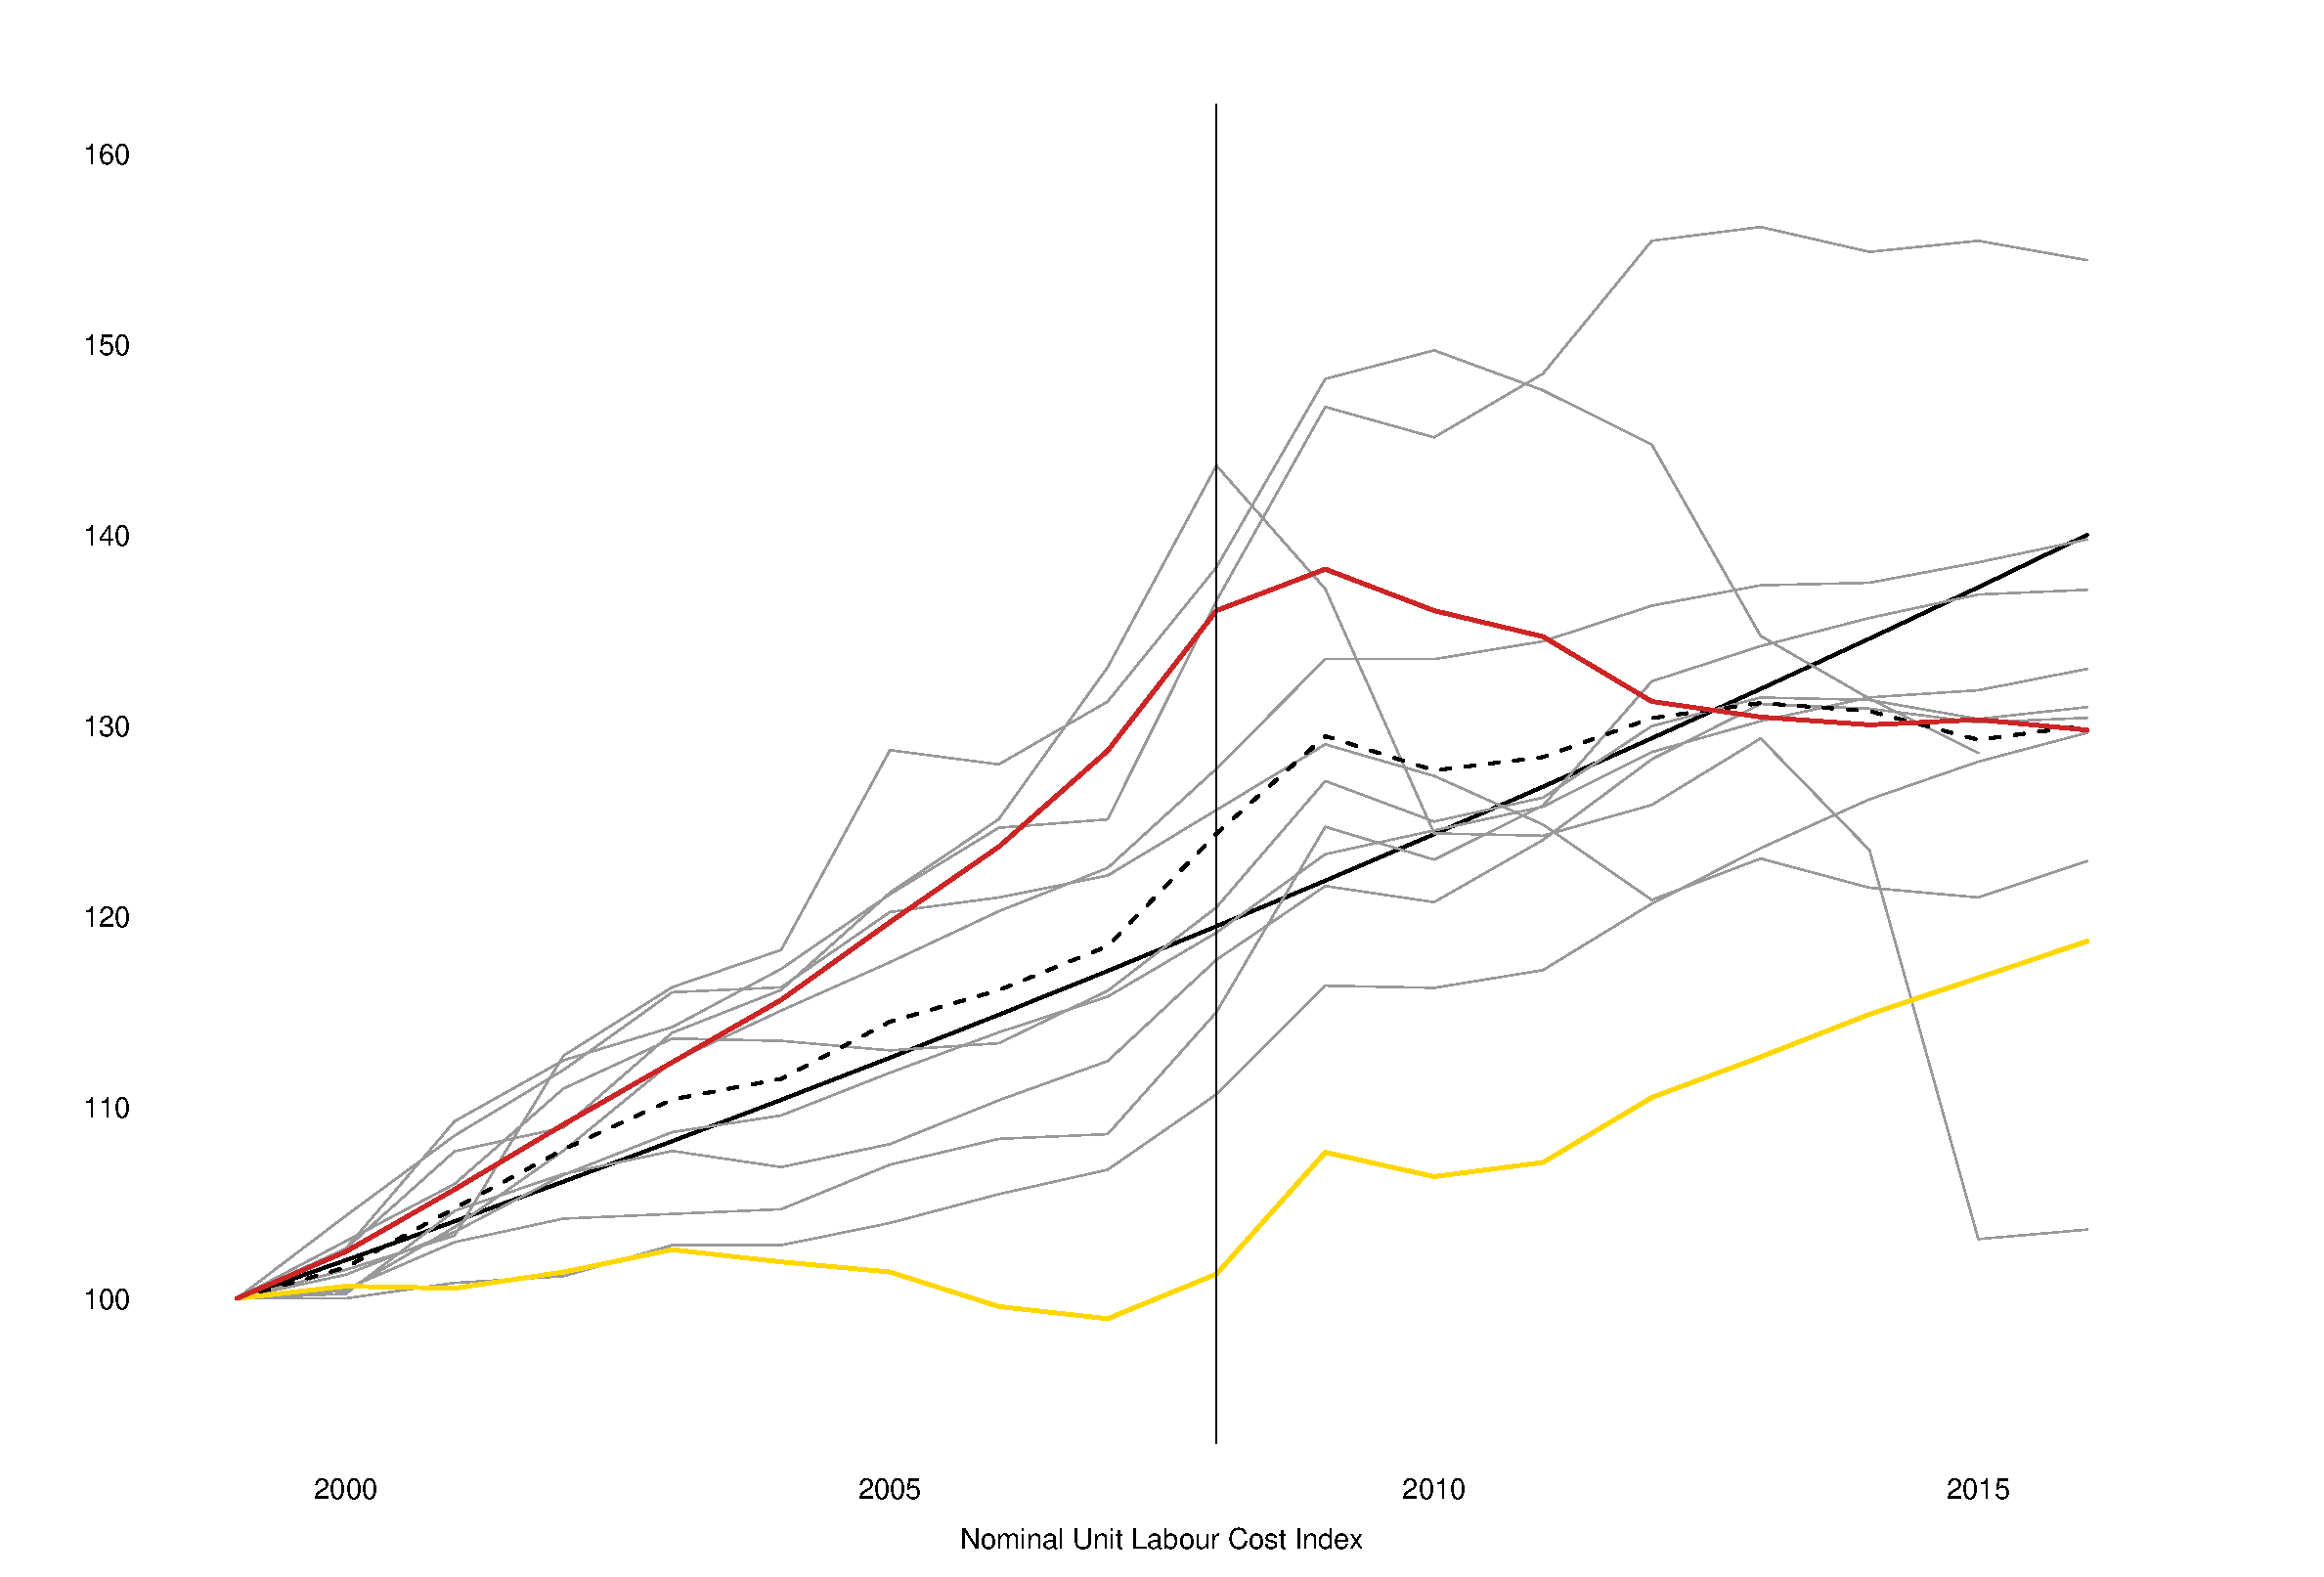
\includegraphics[scale=.3]{unit_labour_cost.eps}
  \end{figure}
\end{frame}
%--------------------------------------

%--------------------------------------
\begin{frame}
  \begin{figure}
    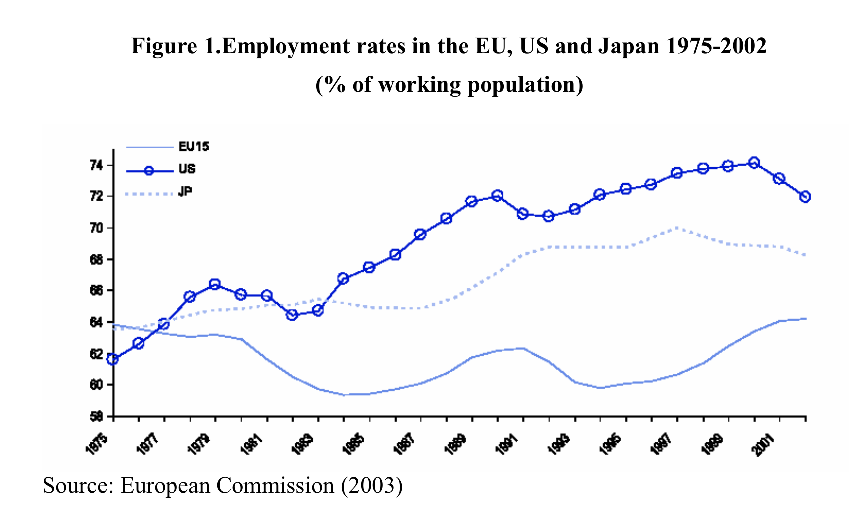
\includegraphics[scale=.7]{employment_rate.eps}
  \end{figure}
\end{frame}
%--------------------------------------

%--------------------------------------
\begin{frame}
  Employment rate is lower because
  \begin{enumerate}
    \item Relatively few new jobs are created
    \item Unemployed Europeans spend more time searching for employment  
  \end{enumerate}
\end{frame}
%--------------------------------------

%--------------------------------------
\begin{frame}
  Besides using US as counterfactual can look at new member states
  \begin{enumerate}
  \item 1970s: Denmark, the United Kingdom, and Ireland 
  \item 1980s: Inclusion of former military regimes; Greece, Portugal, and Spain
  \item 1995: Joining of non-aligned countries after the end of the Cold War in 1995; Austria, Finland, and Sweden
  \item 2000s: Former East Bloc countries joined the EU. 
\end{enumerate} 
\end{frame}
%--------------------------------------

%--------------------------------------
\begin{frame}
  \begin{figure}
    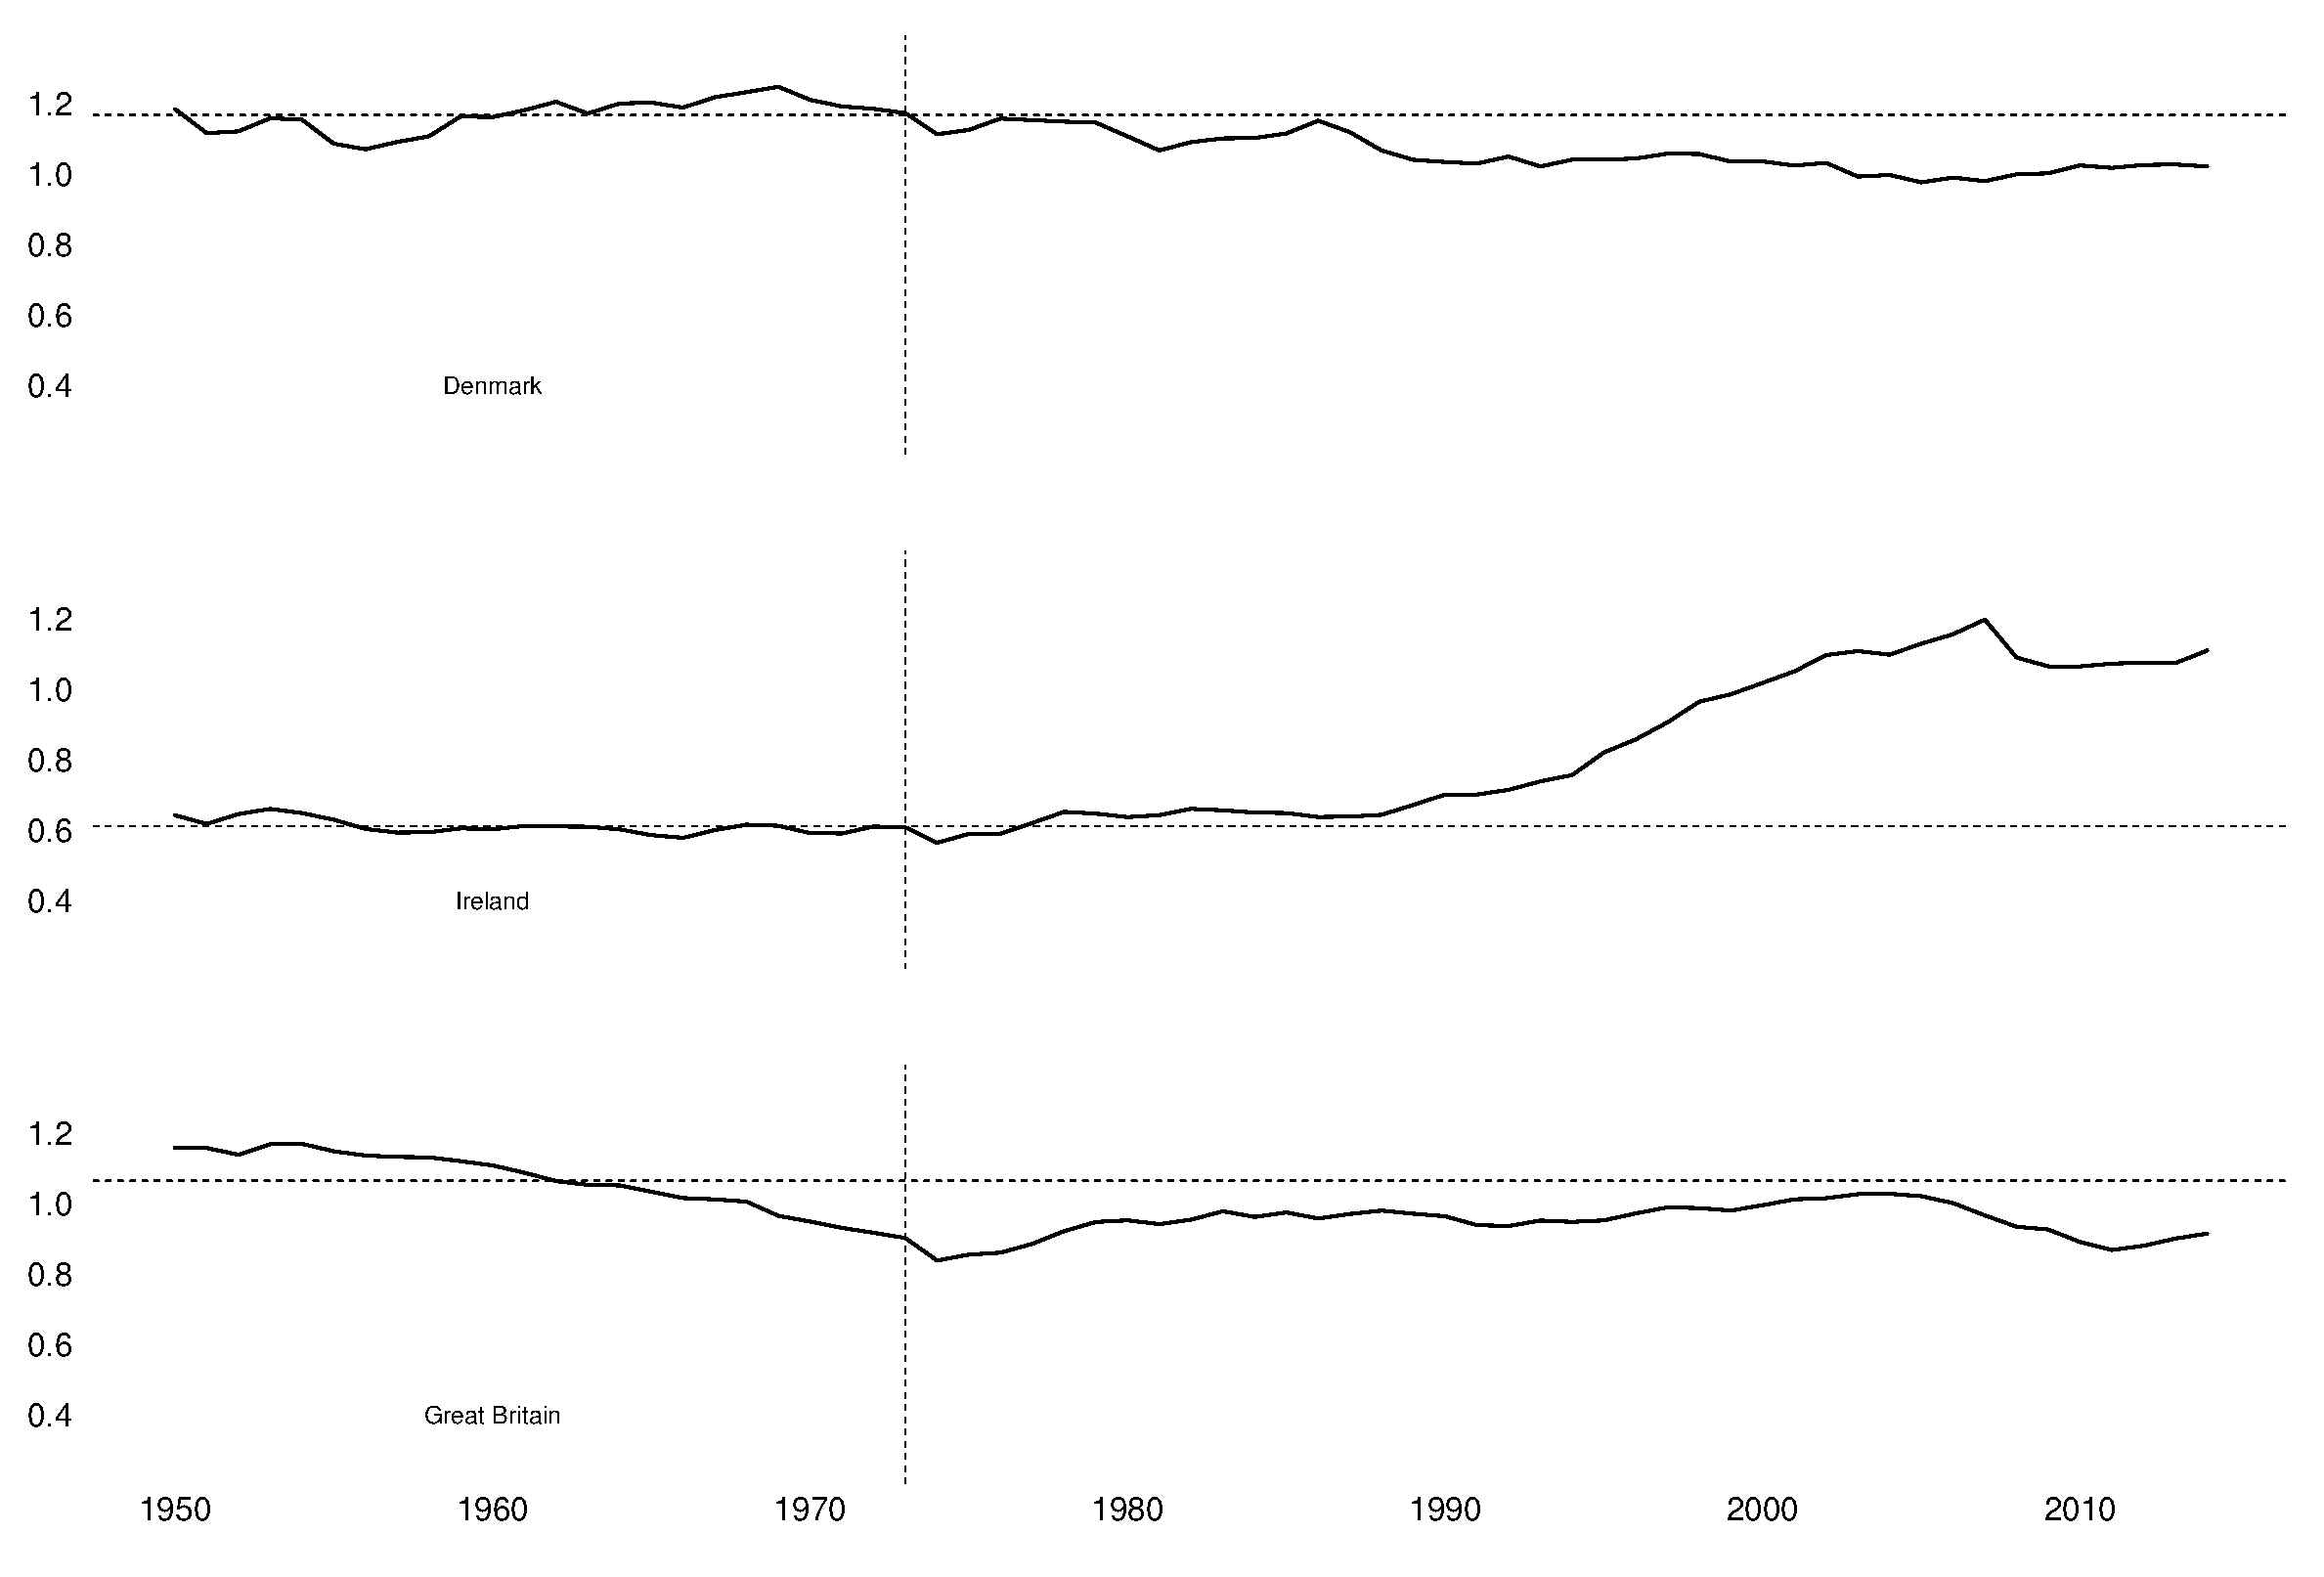
\includegraphics[scale=.3]{enlargement1.eps}
  \end{figure}
\end{frame}
%--------------------------------------

%--------------------------------------
\begin{frame}
  \begin{figure}
    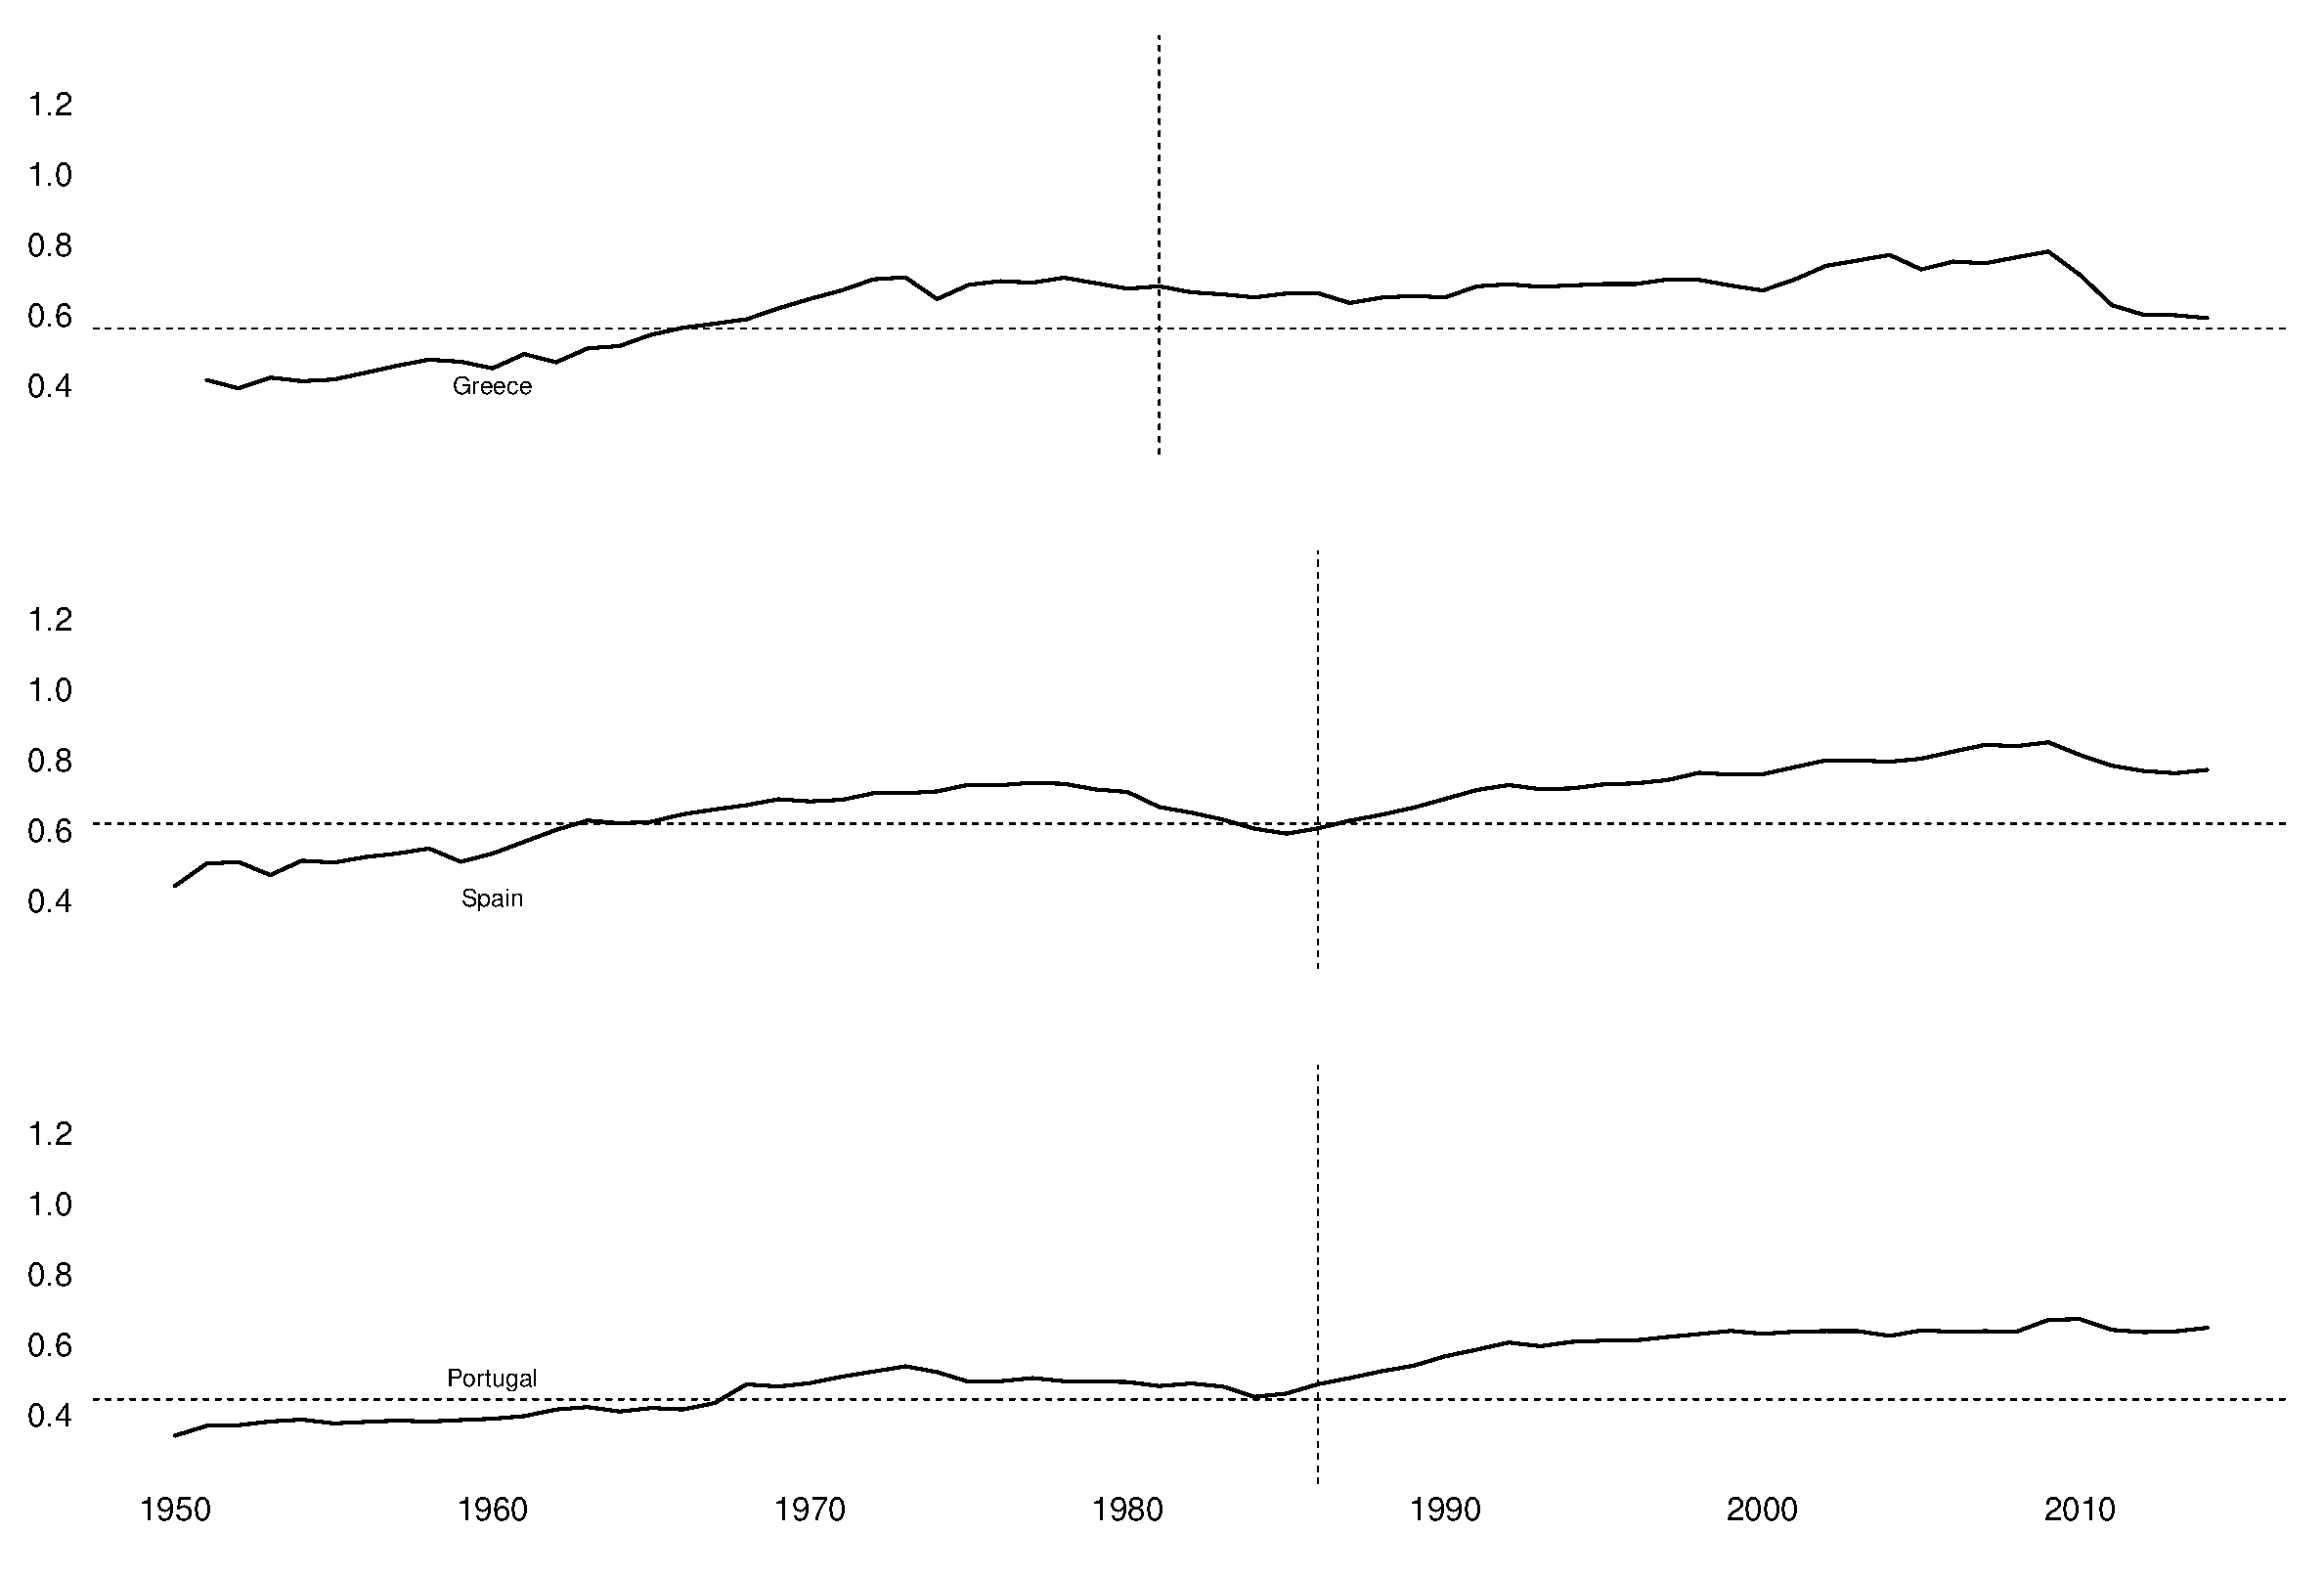
\includegraphics[scale=.3]{enlargement2.eps}
  \end{figure}
\end{frame}
%--------------------------------------

%--------------------------------------
\begin{frame}
  \begin{figure}
    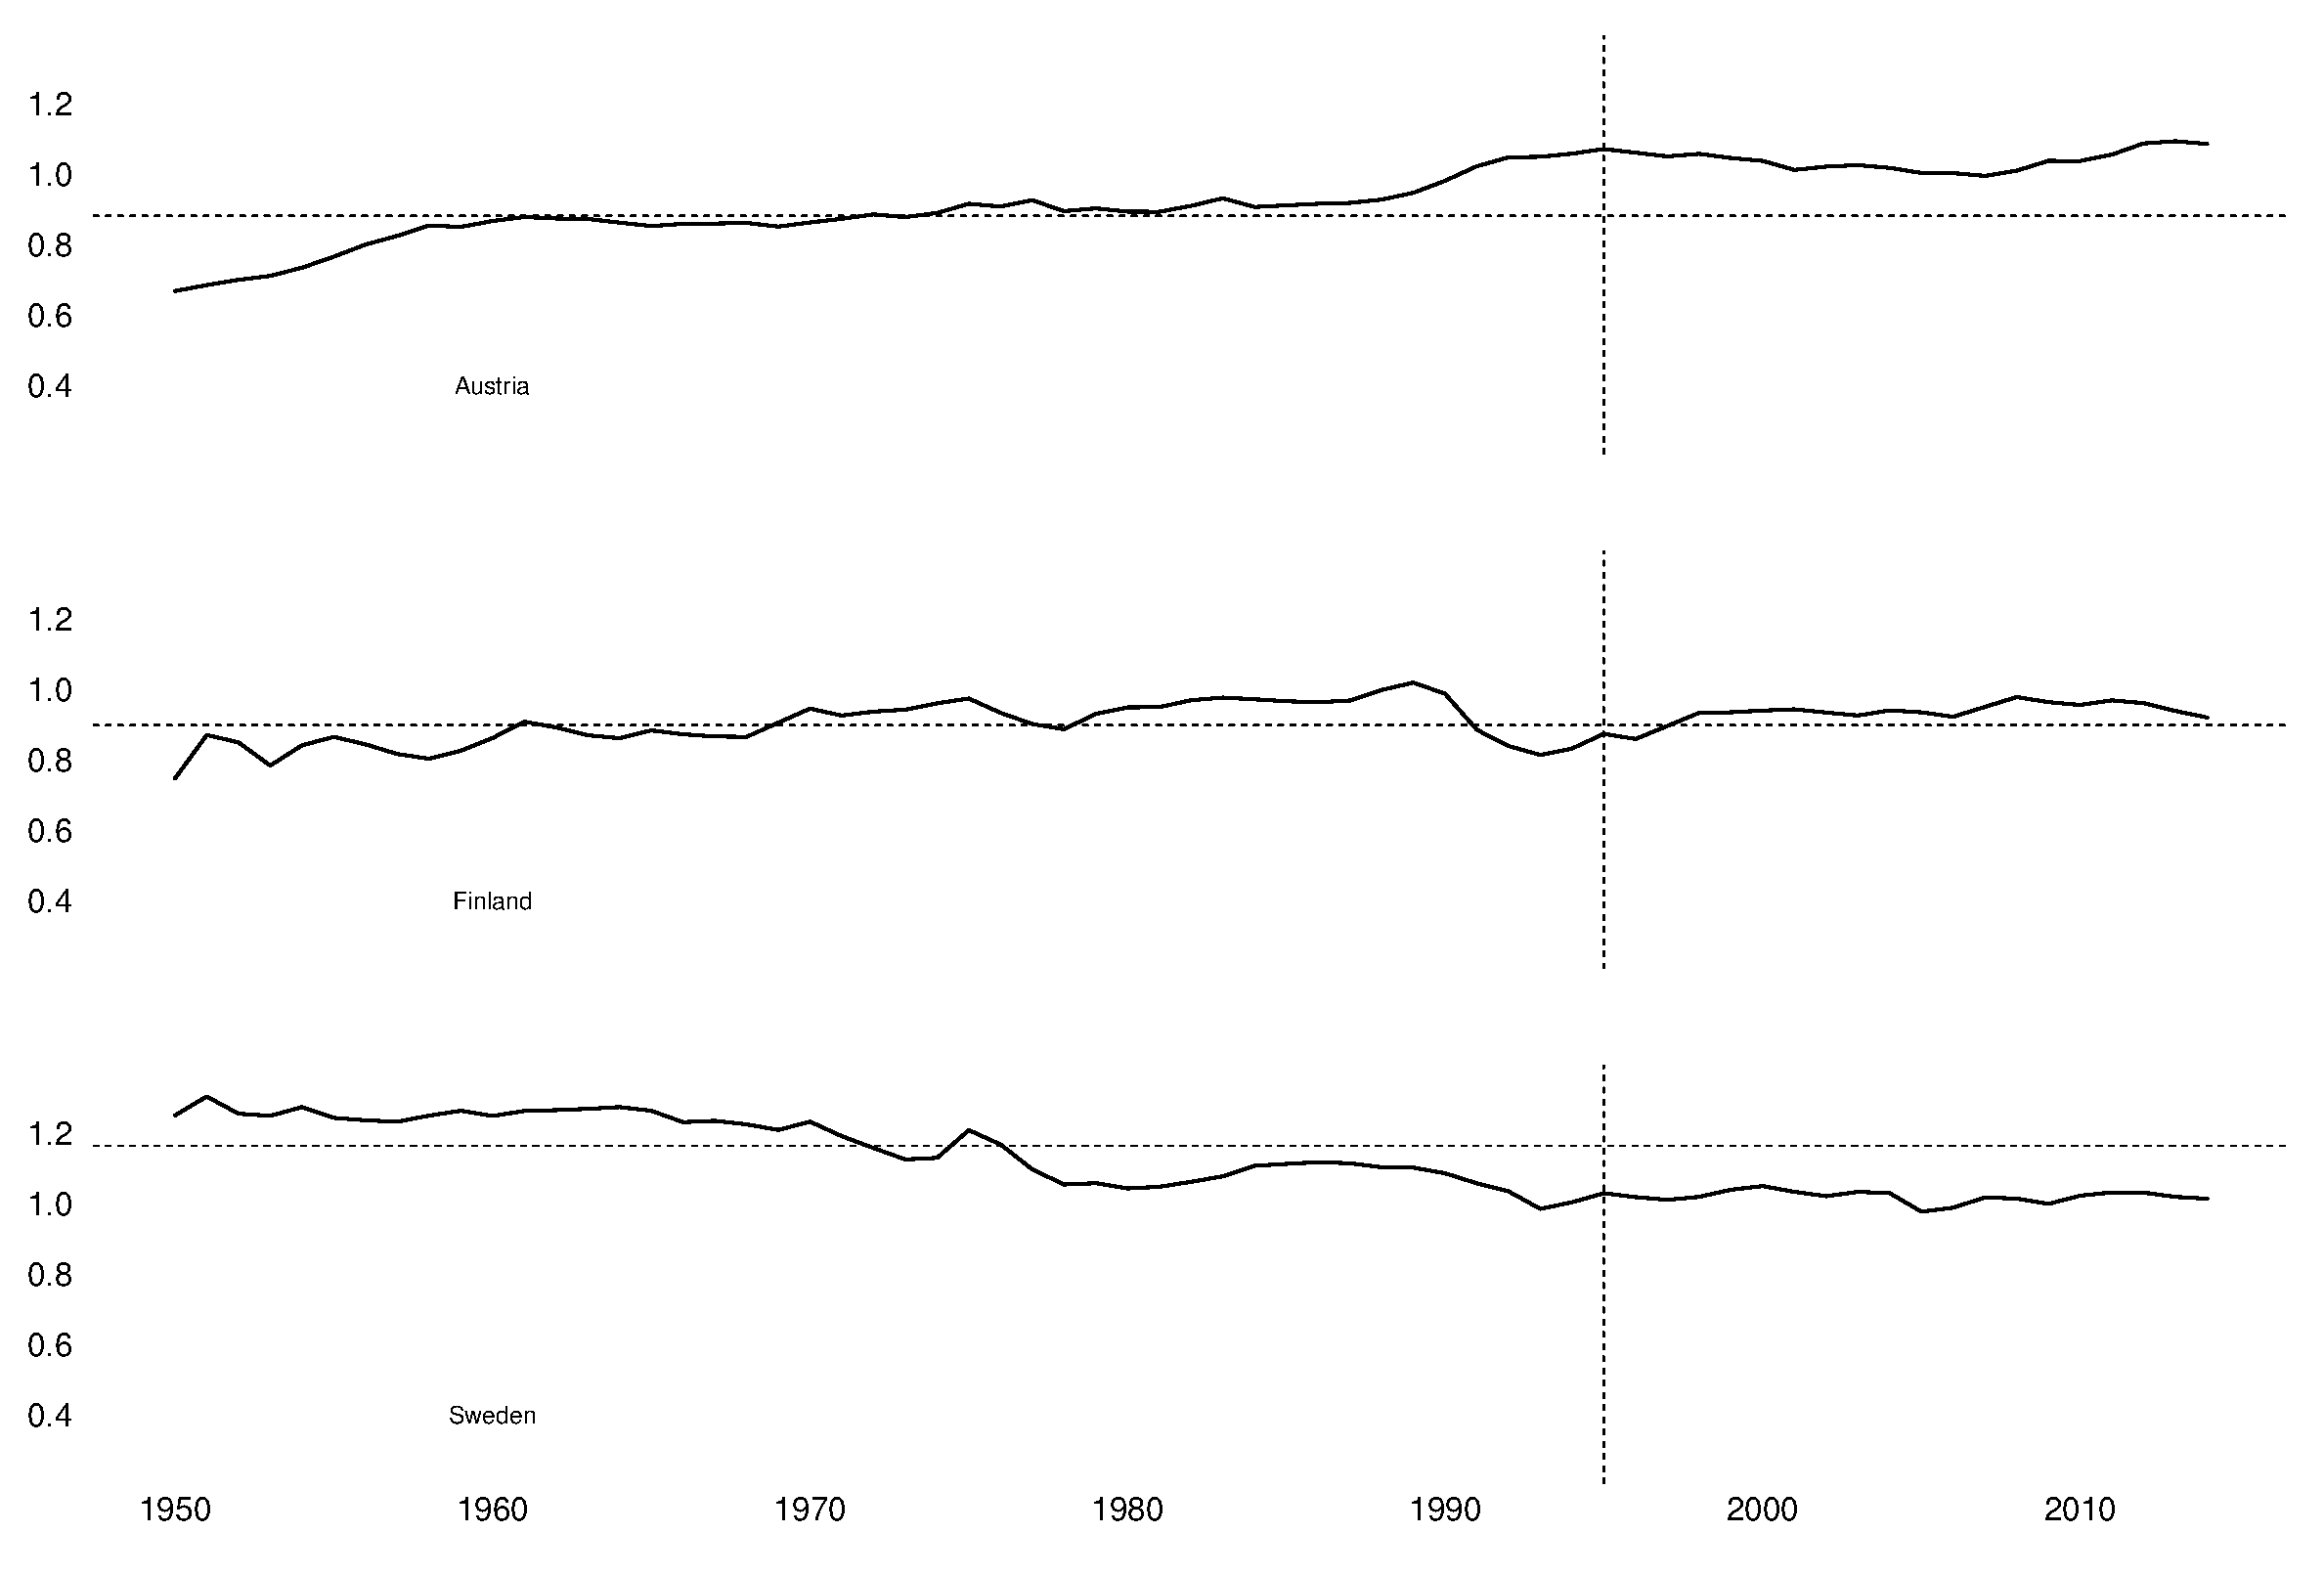
\includegraphics[scale=.3]{enlargement3.eps}
  \end{figure}
\end{frame}
%--------------------------------------

%--------------------------------------
\begin{frame}
  \begin{figure}
    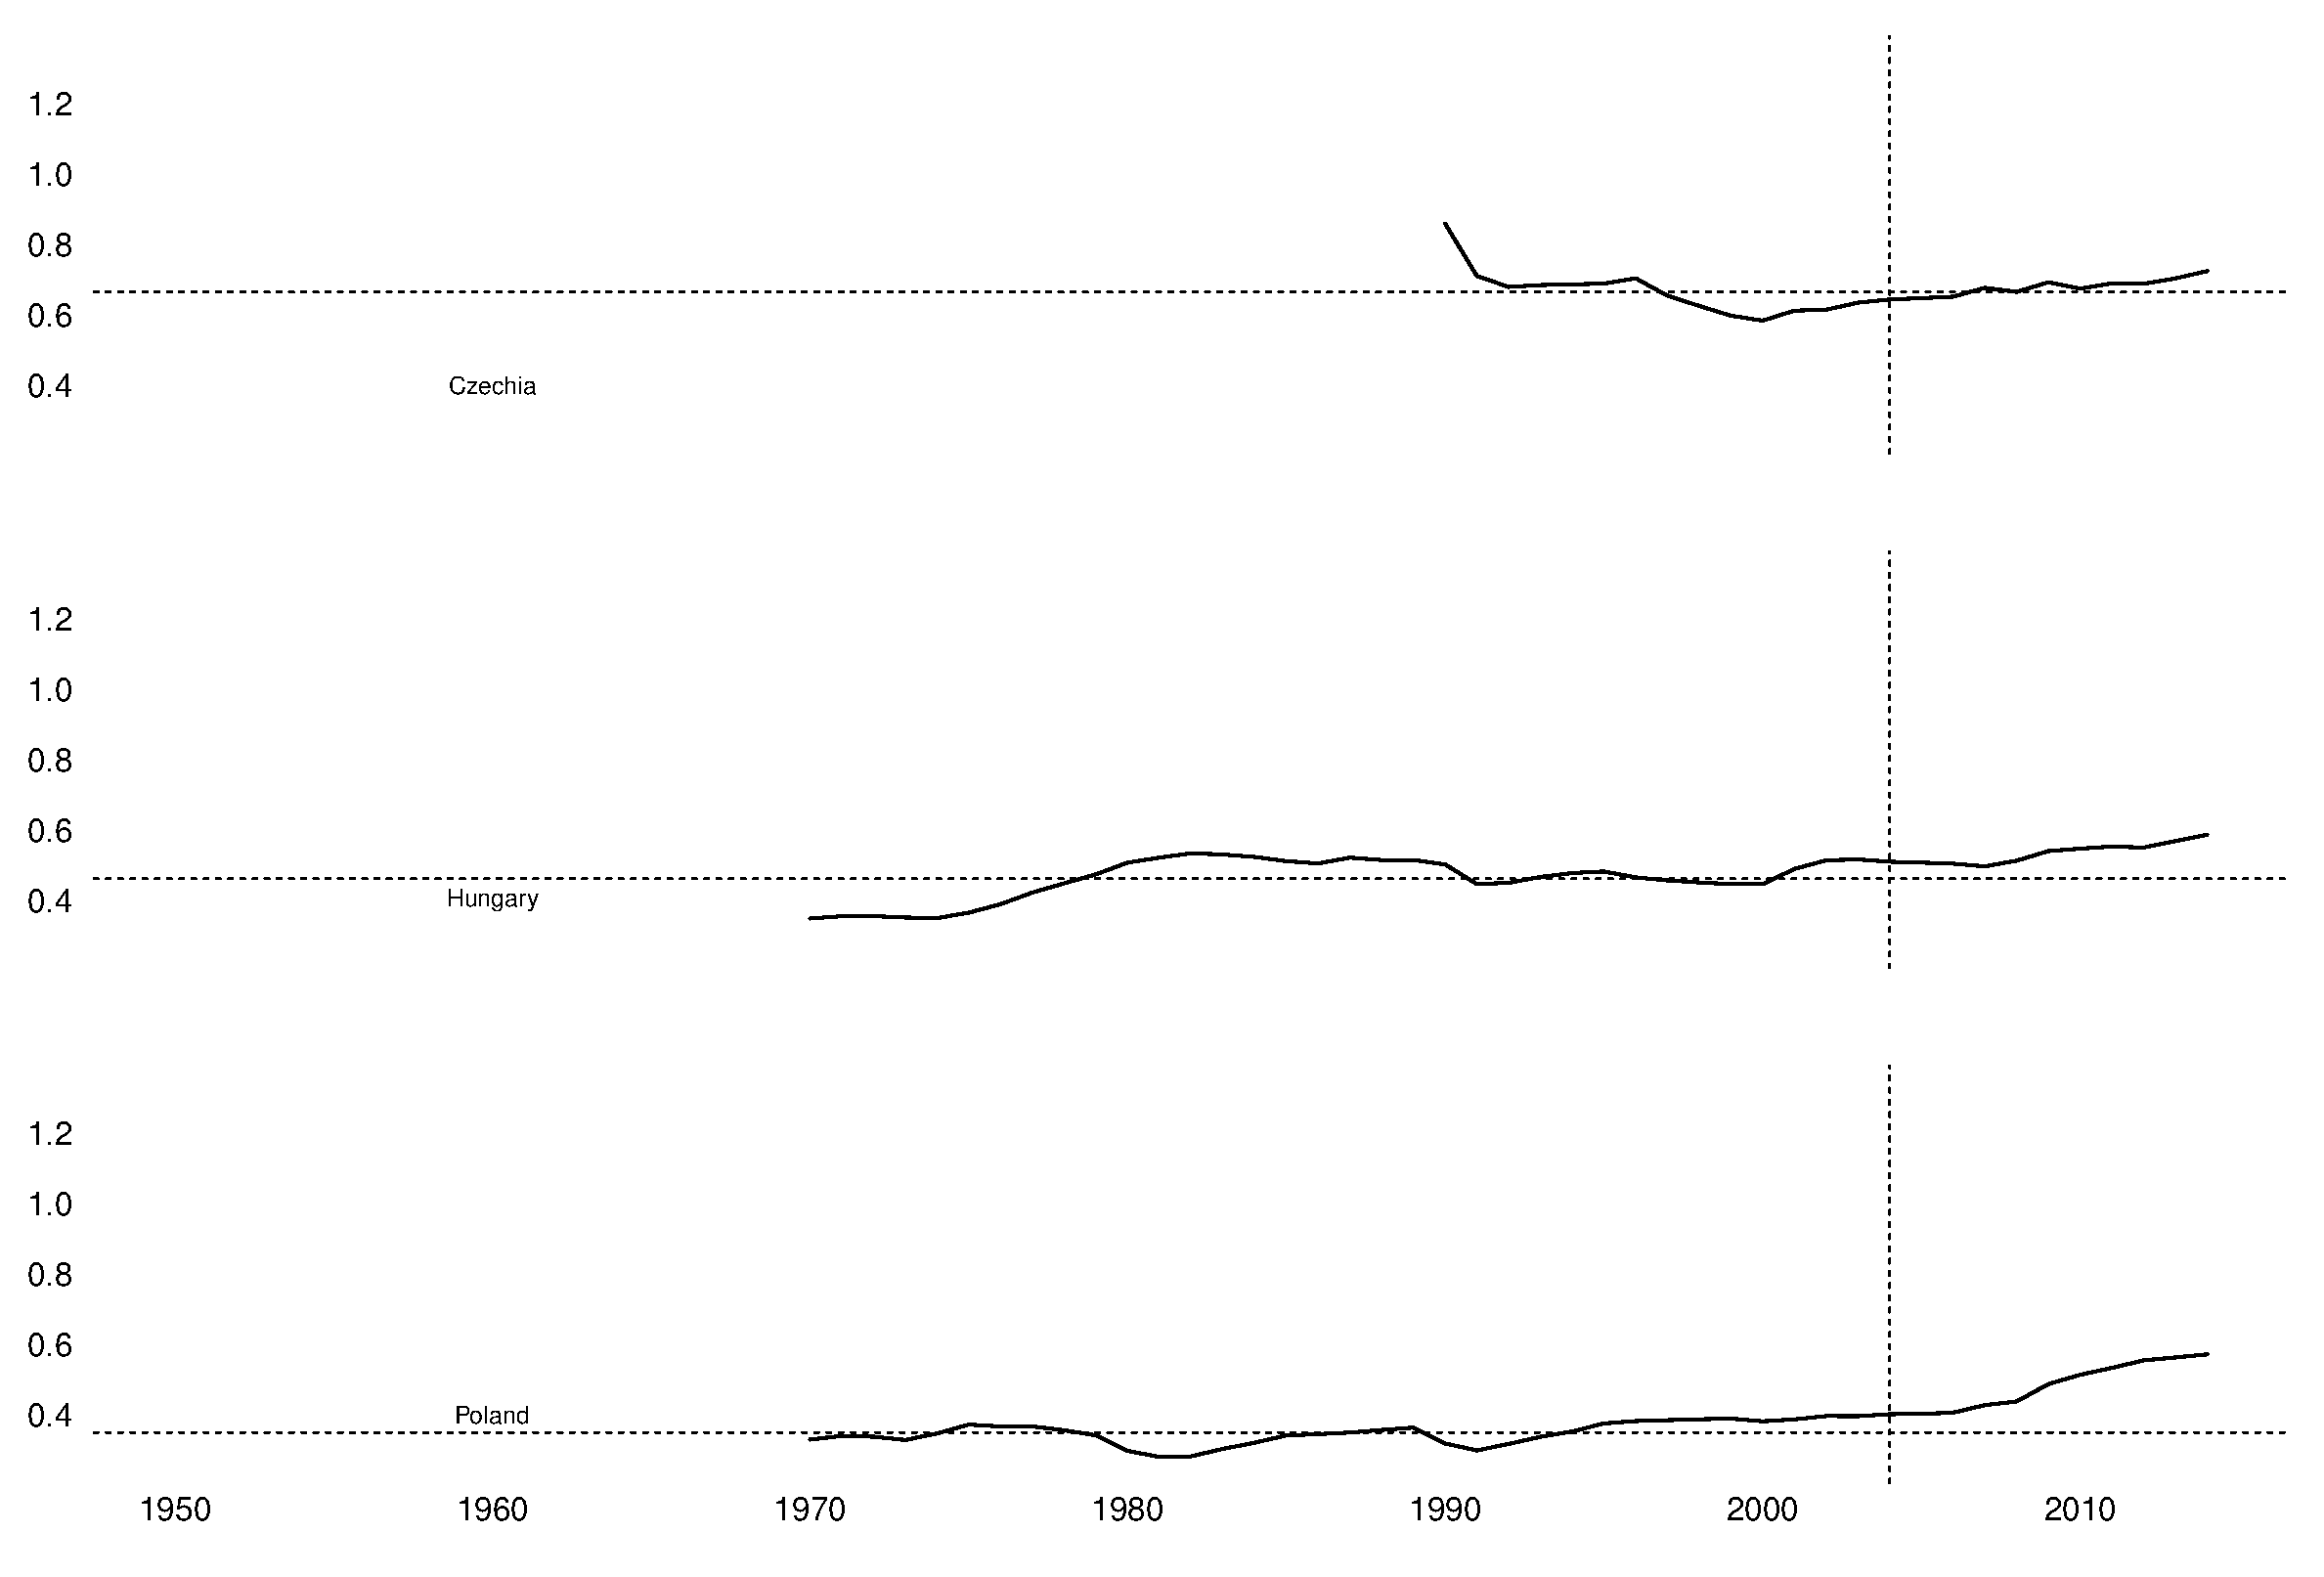
\includegraphics[scale=.3]{enlargement4.eps}
  \end{figure}
\end{frame}
%--------------------------------------



%--------------------------------------
\begin{frame}
  In 2005 evaluation was made on performance of countries that joined in 1995\\
  \textbf{Austria}
  \begin{itemize}
    \item Lower prices resulting in 2\% welfare effect
    \item Additional 0.5\% GDP growth annually
  \end{itemize}
  \textbf{Finland}
  \begin{itemize}
    \item Increase in trade and investment
    \item Lower consumer prices
    \item Large overall impact on economy
  \end{itemize}
  \textbf{Sweden}
  \begin{itemize}
    \item Estimated 0.4\% increase in trend growth
    \item Increase in competition and FDI
    \item Improvement in fiscal and monetary policy
  \end{itemize}
  \medskip
  In general evaluation showed that joining the EU had been beneficial. 
\end{frame}
%--------------------------------------

%--------------------------------------
\begin{frame}
  \textbf{Growth accounting}
  \begin{align}
    G_t^Y=G_t^A + \alpha G_t^K + (1-\alpha)G_t^L
  \end{align}  
  \medskip
  Growth in output equals technology growth plus weighted average of capital and labour growth rates
  \begin{itemize}
    \item Weight determined by $\alpha$
  \end{itemize}
\end{frame}
%--------------------------------------

%--------------------------------------
\begin{frame}
  \begin{figure}
    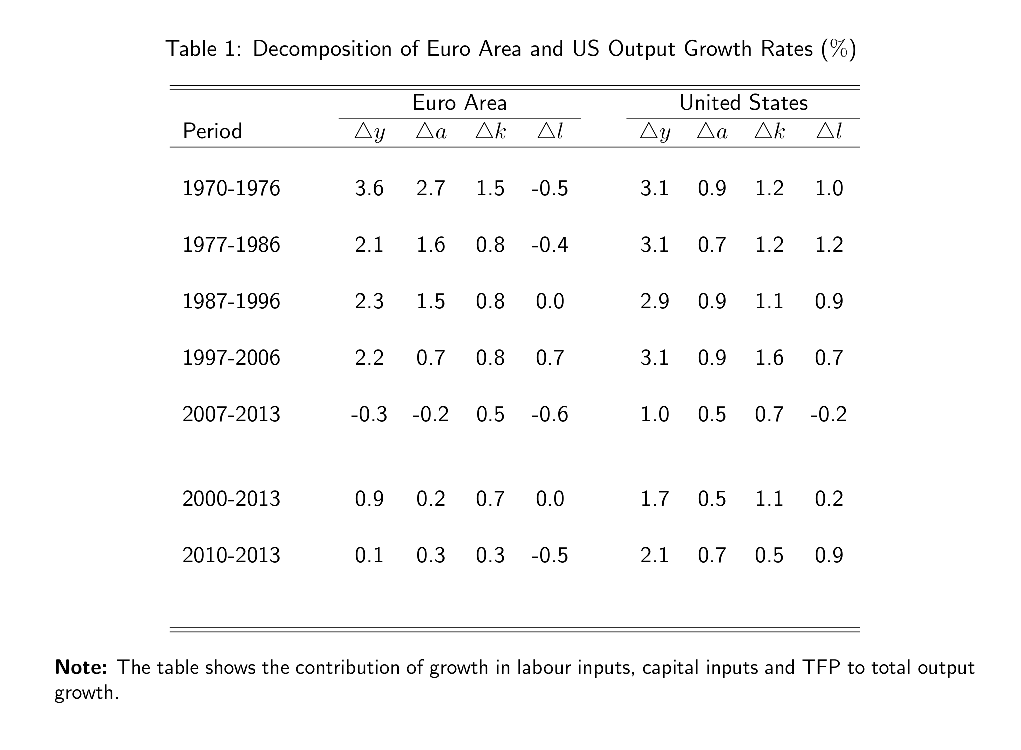
\includegraphics[scale=.7]{growth_accounting1.eps}
  \end{figure}
\end{frame}
%--------------------------------------

%--------------------------------------
\begin{frame}
  \begin{figure}
    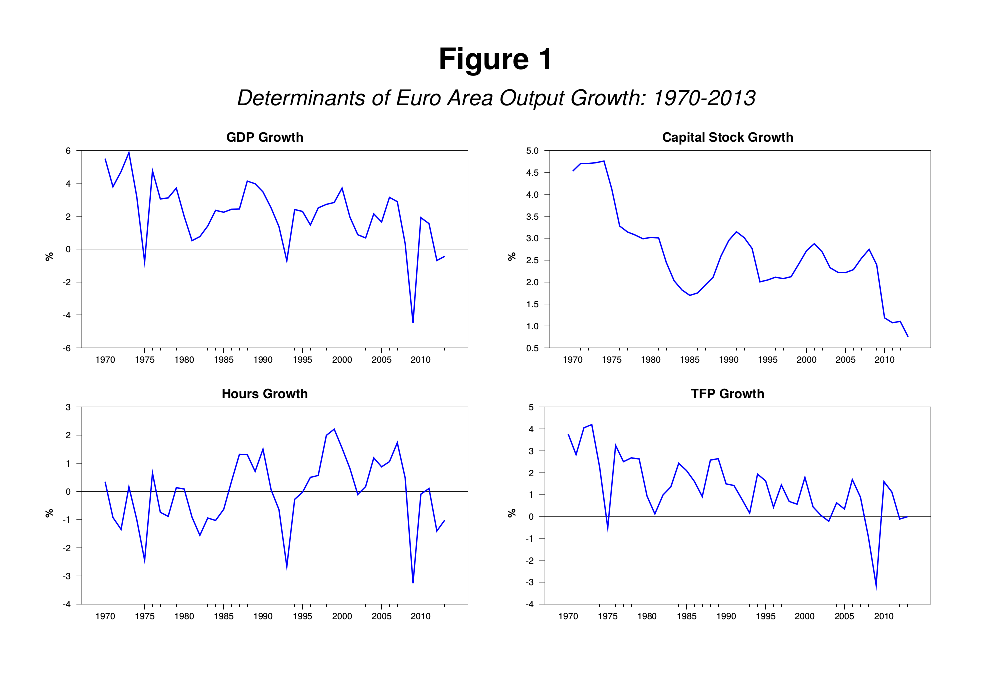
\includegraphics[scale=.7]{growth_accounting2.eps}
  \end{figure}
\end{frame}
%--------------------------------------

%--------------------------------------
\begin{frame}
  \textbf{Europe vs. US}\\
  Growth has been similar but since 1990s US growth has been 1.3 percentage points higher
  \begin{itemize}
    \item Output per worker has declined in Europe
    \item Reduction in TFP growth
  \end{itemize}
  \medskip
  Past output growth relied mainly on increases in
  \begin{itemize}
    \item Capital
    \item Labour
  \end{itemize}
  \medskip
  Less on improvements in TFP: problematic as capital is endogenous.
\end{frame}
%--------------------------------------

%--------------------------------------
\begin{frame}
  \begin{figure}
    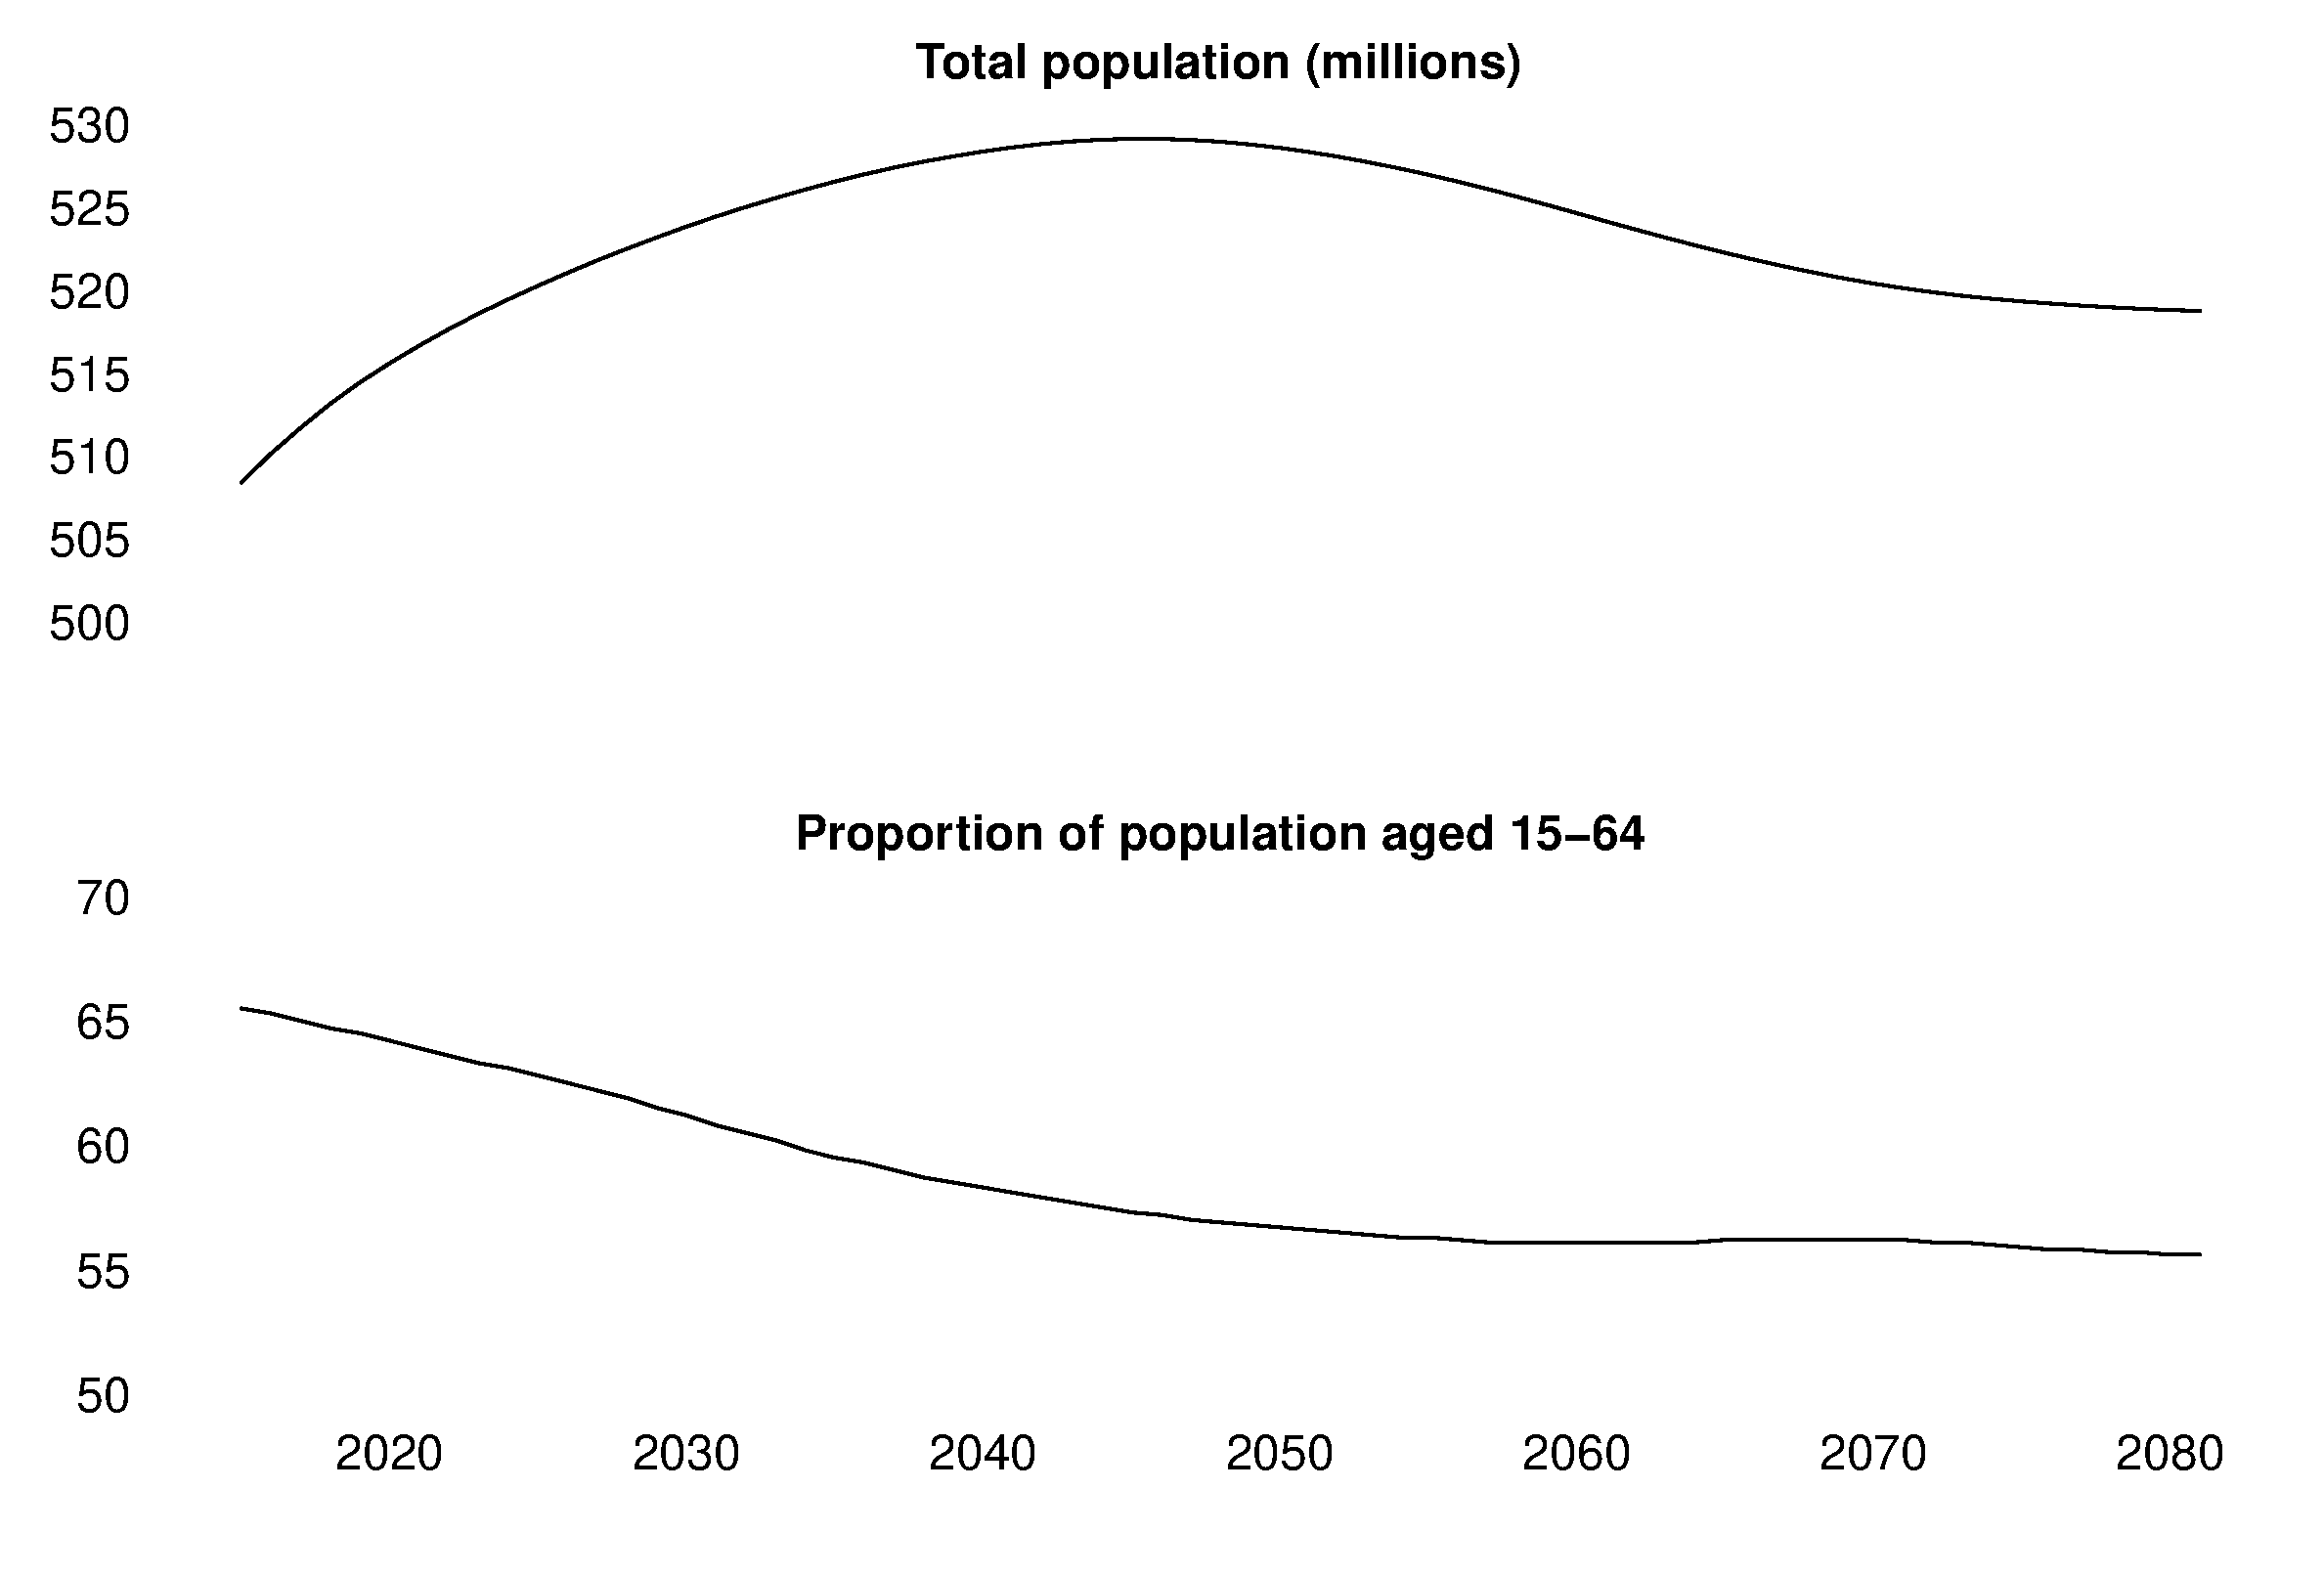
\includegraphics[scale=.3]{population.eps}
  \end{figure}
\end{frame}
%--------------------------------------

%--------------------------------------
\begin{frame}
  Besides TFP slump aging of population is another serious issue
  \begin{itemize}
    \item Population growth is slowing down; expected to peak middle of century
    \item Working population (15-64 years) already peaked
  \end{itemize}
  \medskip
  Probably leads to further reduction in number of hours worked, reducing output growth
  \begin{itemize}
    \item Assuming that the employment rate returns to pre-crisis levels
  \end{itemize}
\end{frame}
%--------------------------------------


%--------------------------------------
\begin{frame}
 Europe's macroeconomic problems are twofold
  
\begin{enumerate}
  \item Short term
  \begin{itemize}
    \item Weak aggregate demand
    \item High levels of public and private debt
  \end{itemize}
  \medskip
  \item Long term
  \begin{itemize}
    \item Demographic challenges  
  \end{itemize}    
\end{enumerate}
\end{frame}
%--------------------------------------

%--------------------------------------
\begin{frame}
  \textbf{Structural reforms} are required to boost productivity, in areas such as
  \begin{enumerate}
  \item Labour market
  \begin{itemize}
    \item Reducing long-run unemployment rates
    \item e.g. protection against dismissals, regulation of part-time work
  \end{itemize}
  \item Pension
  \begin{itemize}
    \item Workers can work to a later age
    \item Similar to Switzerland where there is a relatively high rate of labour participation among older workers
  \end{itemize}
  \item Broader regulatory reforms
  \begin{itemize}
    \item e.g. taxes, education policies, etc. 
  \end{itemize}
\end{enumerate}
\end{frame}
%--------------------------------------

%--------------------------------------
\begin{frame}
  2000 \textbf{Lisbon strategy} aimed to address some of these issues by deregulation of
  \begin{itemize}
    \item Labour markets
    \item Product markets
  \end{itemize}
  \medskip
  Aim was to create
  \begin{quote}
    the most dynamic, knowledge based economy in the world by 2010  
  \end{quote}
  \medskip
  Failed  
\end{frame}
%--------------------------------------

%--------------------------------------
\begin{frame}
  Lisbon strategy focused specifically on 
  \begin{itemize}
  \item Problems posed by the public sector
  \begin{itemize}
    \item Risk-taking was discouraged by large bureaucracies
    \item Public services that are often inefficient
    \item Policies that protect jobs rather than people
  \end{itemize}
  \item Salience of national interests
  \begin{itemize}
    \item Protectionist measures that inhibit competition in the services sector
    \item Absence of unified research space
  \end{itemize}
\end{itemize}
\end{frame}
%--------------------------------------

%--------------------------------------
\begin{frame}
  \textbf{Europe 2020}\\
  New 10-year strategy rolled out in 2010
  \begin{itemize}
    \item Strategy identified that the responsibility for structural reforms lies with the national governments 
    \item But should rely on the European single market and the common trade policy
  \end{itemize}  
\end{frame}
%--------------------------------------

%--------------------------------------
\begin{frame}
  Europe 2020 key issues\\
  \textbf{Employment}
  \begin{itemize}
    \item Target of 75\% employment rate of 20-64-year-olds
  \end{itemize}

  \textbf{Innovation}
  \begin{itemize}
    \item Invest 3\% of EU's GDP in R and D
  \end{itemize}
  
  \textbf{Climate/energy}
  \begin{itemize}
    \item Limit greenhouse gasses by 20-30\% compared to 1990 levels
    \item 20\% of energy requirements coming from renewable energy
    \item Increasing energy efficiency by 20\%
  \end{itemize}
  
  \textbf{Education}
  \begin{itemize}
    \item Reduce school dropout rate below 10\%
    \item 40\% of 30-34 years old completing tertiary education
  \end{itemize}
  
  \textbf{Social inclusion}
  \begin{itemize}  
    \item Reduce people at risk of poverty or social exclusion with 20 million
  \end{itemize}
\end{frame}
%--------------------------------------

%--------------------------------------
\end{document}
